\documentclass{beamer}
%\documentclass[notes]{beamer}       % print frame + notes
%\documentclass[notes=only]{beamer}   % only notes
%\documentclass{beamer}              % only frames

\usepackage[latin1]{inputenc}
\usetheme{Warsaw}
\setbeamertemplate{headline}{%
\leavevmode%
  \hbox{%
    \begin{beamercolorbox}[wd=\paperwidth,ht=2.5ex,dp=1.125ex]{palette quaternary}%
    \insertsectionnavigationhorizontal{\paperwidth}{}{\hskip0pt plus1filll}
    \end{beamercolorbox}%
  }
}

\title{A Comparative study of Different Predictor Concepts on a HWI Data Set}
\author{Marc Wildi}
\institute{Institute of data analysis and process design (ZHAW)}
\date{May, 2024}
\date[\today]{}

\usepackage{Sweave}
\begin{document}

\begin{frame}
\titlepage
\end{frame}




\begin{frame}[allowframebreaks]{Table of Contents}
\tableofcontents
\end{frame}


\section{Introduction}



\begin{frame} {Introduction}
\begin{itemize}
\item See slides on ip (ip-case) for a similar introduction: motivation of trends vs. direct forecasts and theses
\end{itemize}
\end{frame}


\begin{frame} {Zero-crossings BIP: Standardized Series}
\begin{figure}[H]\begin{center}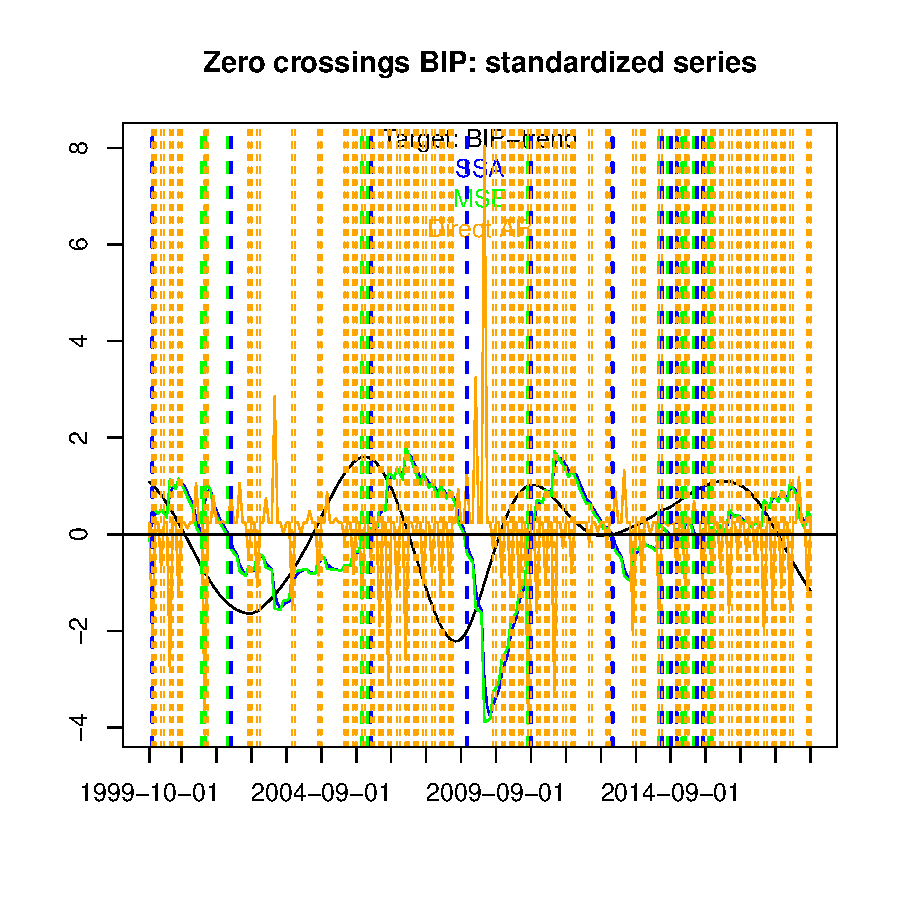
\includegraphics[height=3in, width=4.5in]{zero_cross_ifo_l_1.pdf}\caption{\label{data}}\end{center}\end{figure}\end{frame}






\begin{frame} {Overview of (and Links to) Performance Metrics in this Study}
\begin{itemize}
\item Relative \textbf{forecast mean-square} error (target: BIP-shifted): slide \eqref{rmse1} (direct AR forecasts full sample), \eqref{rmse2} (same but shorter sample), \eqref{rmse3} (univariate filters, full sample), \eqref{rmse4} (same but before Pandemic), \eqref{slide_multi_rel_mse} (multivariate filters) 

\item Relative \textbf{filter mean-square} error (target: BIP-trend): \eqref{rfmse1} (outperformance of multivariate over univariate)

\item Target \textbf{correlations}: \eqref{sample_target_cor1}, \eqref{sample_target_cor2}, \eqref{sample_target_cor3} and \eqref{sample_target_cor4} 

\item \textbf{Sign accuracies}: \eqref{signaac1} and \eqref{signaac2}

\item \textbf{t-statistics}: \eqref{tstat1},  (univariate filters and direct AR, full sample), \eqref{tstat2} (same but prior pandemic), \eqref{slide_multi_rel_mse} (multivariate filters)

\item \textbf{Holding times}: \eqref{htzc1} (direct AR and univariate filters), \eqref{htzc2} and \eqref{htzc3} (M-SSA vs. M-MSE)
\end{itemize}
\end{frame}




\section{Data}

\frame{\sectionpage}












\begin{frame} {Data}

\subsection{Ragged End}


\begin{itemize}
\item Selected (small) data set: BIP,ip,ifo-c,ifo-exp,ifo-l,ESI,spr-10y-3m (we did not consider pmi because the series is shorter: for consistency we thus would have to shorten the evaluation span: pmi is OK but not best overall)
\item Transformations: 
\begin{itemize}
\item log returns (except spread which is differenced only) 
\item scaling (we mostly work with standardized series)
\item trim scaled data to $\pm 5$ (to regularize singular pandemic data)
\end{itemize}
\item Target: BIP (shifted by forecast horizon and publication lag, see below)
\item Explanatories: see the above selection 
\item Ragged end: see below 
\end{itemize}
\end{frame}


\begin{frame} {Ragged End}
\begin{itemize}
\item Ragged end: prior to shifting:
% latex table generated in R 4.2.2 by xtable 1.8-4 package
% Sat Feb 15 08:35:27 2025
\begin{table}[ht]
\centering
\begin{tabular}{rrrrrrrr}
  \hline
 & BIP & ip & ifo\_c & ifo\_exp & ifo\_l & ESI & spr\_10y\_3m \\ 
  \hline
2024-09-01 &  & 91.20 & 83.70 & 85.90 & 81.60 & 89.80 & -1.40 \\ 
  2024-10-01 & 900.76 & 90.80 & 84.10 & 87.50 & 80.80 & 90.70 & -1.20 \\ 
  2024-11-01 &  & 92.20 & 83.80 & 86.80 & 81.00 & 89.30 & -0.90 \\ 
  2024-12-01 &  &  & 82.80 & 84.80 & 80.90 & 86.90 & -0.80 \\ 
  2025-01-01 &  &  & 82.50 & 83.20 & 81.70 & 88.10 & -0.20 \\ 
  2025-02-01 &  &  &  &  &  &  & -0.20 \\ 
   \hline
\end{tabular}
\caption{Ragged end } 
\label{perf_var1}
\end{table}\item Findings:
\begin{itemize}
\item Publication lags: lag(BIP)=4, lag(ip) =2, lag(ESI)=1 (same as pmi); the other variables are contemporaneous
\item Real-time data: shift all series to be aligned at sample end
\item Introduce a new `target' column based on BIP. 
\item Target: real-time BIP shifted by sum of publication lag and forecast horizon $h=3$, i.e., shift=$h+lag=$7
\item Ignore data revisions 

\end{itemize}
\end{itemize}
\end{frame}



\begin{frame} {Real-Time data: Forecast Horizon $h=3$}

\begin{itemize}

\item Real-time data matrix: shift of target depends on forecast horizon $h=3$: 

% latex table generated in R 4.2.2 by xtable 1.8-4 package
% Sat Feb 15 08:35:27 2025
\begin{table}[ht]
\centering
\begin{tabular}{rrrrrrrrr}
  \hline
 & target & BIP & ip & ifo\_c & ifo\_exp & ifo\_l & ESI & spr\_10y\_3m \\ 
  \hline
2024-05-01 & 902.57 & 904.30 & 95.10 & 88.30 & 89.80 & 86.90 & 91.80 & -1.40 \\ 
  2024-06-01 & 902.57 & 904.30 & 94.60 & 89.30 & 90.80 & 87.80 & 92.40 & -1.30 \\ 
  2024-07-01 & 900.76 & 904.30 & 94.70 & 87.60 & 88.20 & 86.90 & 92.20 & -1.30 \\ 
  2024-08-01 & 900.76 & 901.62 & 91.70 & 85.80 & 87.60 & 84.10 & 92.50 & -1.40 \\ 
  2024-09-01 & 900.76 & 901.62 & 93.40 & 84.90 & 86.80 & 83.00 & 90.90 & -1.40 \\ 
  2024-10-01 & 900.76 & 901.62 & 90.70 & 83.70 & 85.90 & 81.60 & 89.80 & -1.20 \\ 
  2024-11-01 & 900.76 & 902.57 & 93.20 & 84.10 & 87.50 & 80.80 & 90.70 & -0.90 \\ 
  2024-12-01 & 900.76 & 902.57 & 91.20 & 83.80 & 86.80 & 81.00 & 89.30 & -0.80 \\ 
  2025-01-01 & 900.76 & 902.57 & 90.80 & 82.80 & 84.80 & 80.90 & 86.90 & -0.20 \\ 
  2025-02-01 & 900.76 & 900.76 & 92.20 & 82.50 & 83.20 & 81.70 & 88.10 & -0.20 \\ 
   \hline
\end{tabular}
\caption{Target column shifted upwards by h+publication lag=7. All other explanatories are shifted to be aligned at sample end.  } 
\label{perf_var1}
\end{table}\end{itemize}

\end{frame}

\subsection{Leads and Lags of `Real-Time' Data}

\begin{frame} {Leads/Lags}
\begin{itemize}
\item Analysis of leads/lags in real-time data matrix
\item Compute cross correlation function (CCF) between target and explanatory variables
\begin{itemize}
\item Peak of CCF indicates lead (left-shift) or lag (right-shift)
\item Note: (shift of) target depends on $h$
\end{itemize}
\end{itemize}
\end{frame}



\begin{frame} {Data and CCF for $h=3$}
\begin{figure}[H]\begin{center}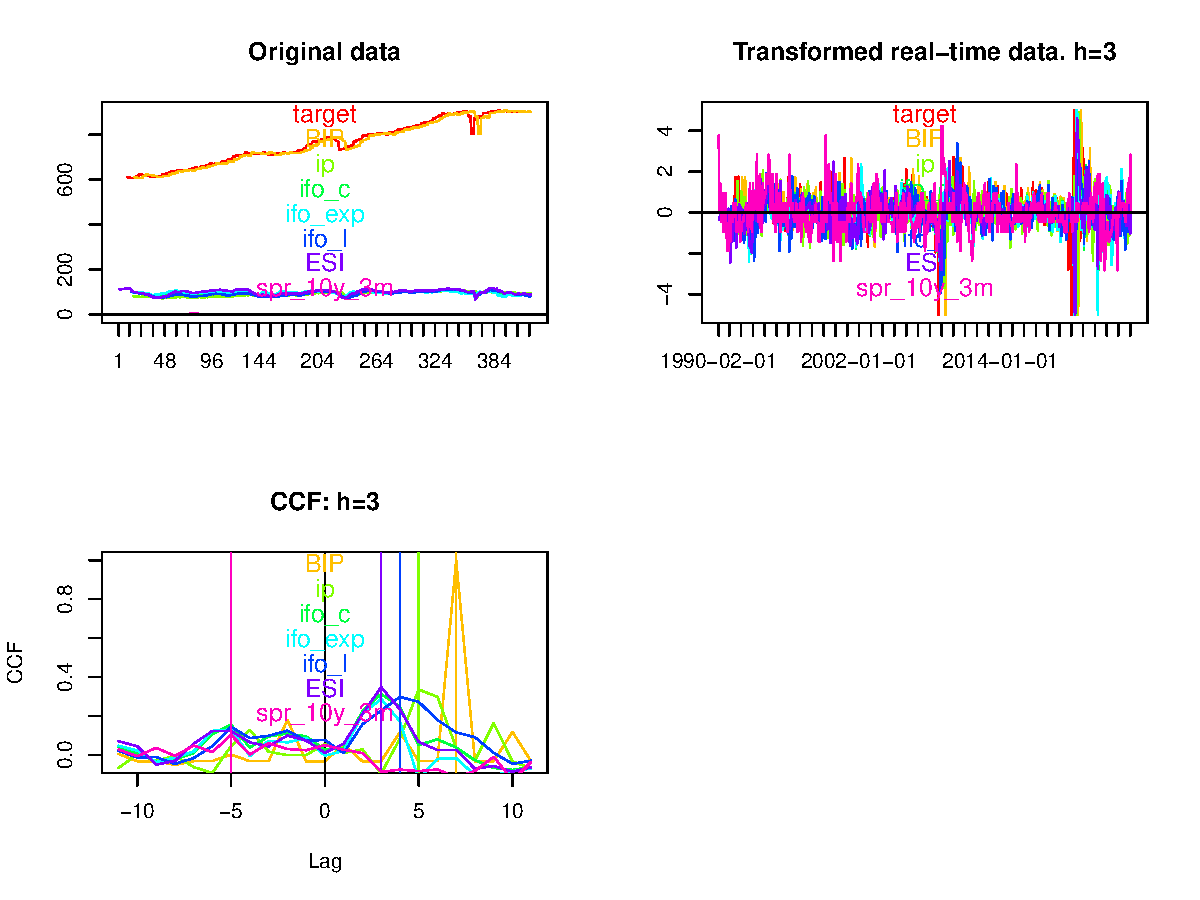
\includegraphics[height=3in, width=4in]{data.pdf}\caption{Selected data: original (top left) and transformed (top right). Cross correlation functions (bottom) \label{cor}}\end{center}\end{figure}\end{frame}

\begin{frame} {CCF for $h=3$}\label{ccf}
\begin{figure}[H]\begin{center}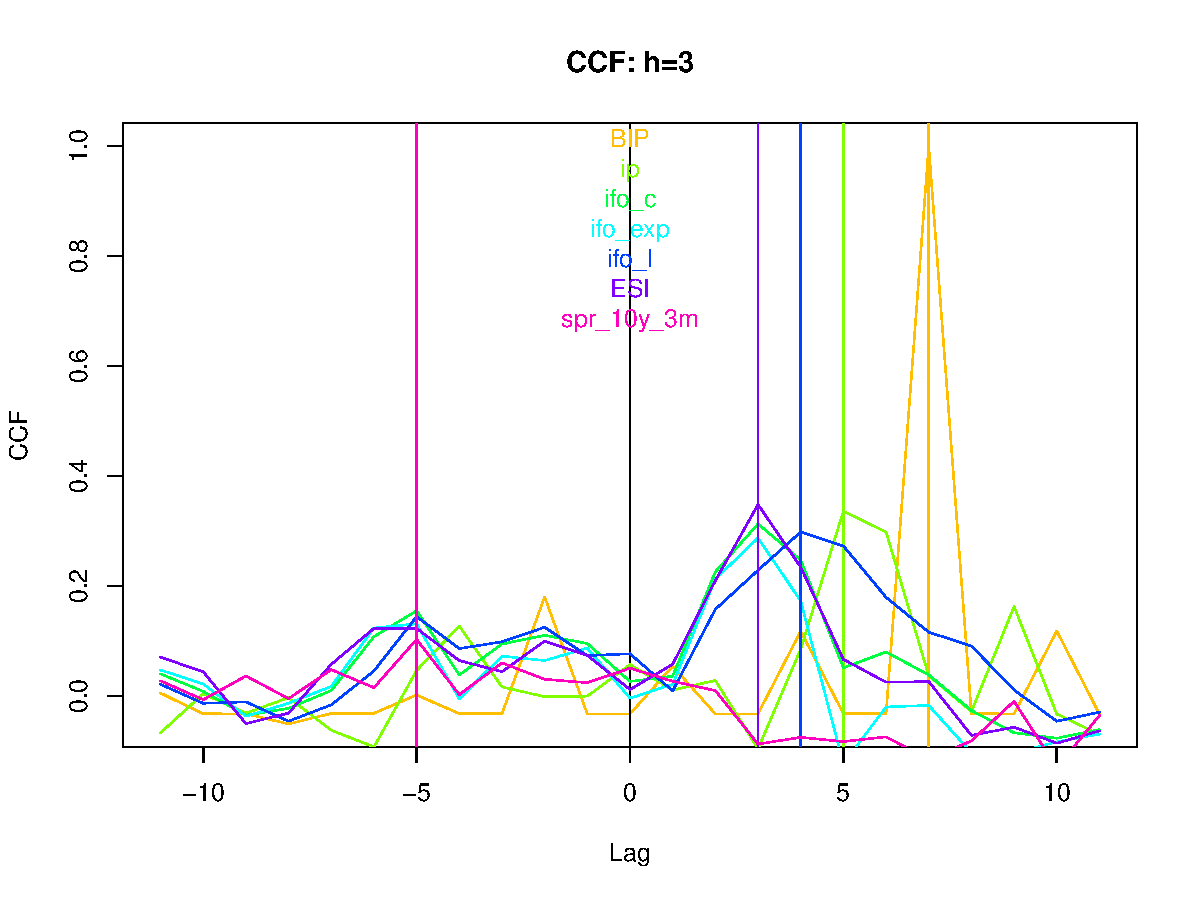
\includegraphics[height=3in, width=4in]{CCF.pdf}\caption{Selected data: original (top left) and transformed (top right). Cross correlation functions (bottom) \label{cor}}\end{center}\end{figure}\end{frame}





\begin{frame} {Leads/Lags}
% latex table generated in R 4.2.2 by xtable 1.8-4 package
% Sat Feb 15 08:35:27 2025
\begin{table}[ht]
\centering
\begin{tabular}{rr}
  \hline
 & Peak correlation \\ 
  \hline
BIP & 7.00 \\ 
  ip & 5.00 \\ 
  ifo\_c & 3.00 \\ 
  ifo\_exp & 3.00 \\ 
  ifo\_l & 4.00 \\ 
  ESI & 3.00 \\ 
  spr\_10y\_3m & -5.00 \\ 
   \hline
\end{tabular}
\caption{Peak correlation: positive numbers signify a lag of the real-time explanatory (shifted backward by its publication lag) relative to the target (shifted forward  by the forecast horizon).} 
\label{perf_var1}
\end{table}
\begin{itemize}
\item Stair-step interpolation of BIP makes an assessment of leads/lags less clear (than for ip)
\end{itemize}
\end{frame}

\subsection{Non-Stationarity: Structural Changes?}

\begin{frame} {Non-Stationarity (Structural Change?)}
\begin{itemize}
\item The \textbf{dependence} structure of some of the series seems to \textbf{change} over time (in particular before/after Pandemic)
\item This can have more or less severe impacts on data \textbf{modelling}, \textbf{filtering}, forecast \textbf{performances}, \textbf{holding times} (to be defined below),...
\item Example: {ACF} of \textbf{ifo-exp} for data prior Pandemic (up to 2019) vs. full data set, see plot on next next 
\end{itemize}
\end{frame}



\begin{frame} {Non-Stationarity/Structural Change in Dependence: ifo-exp}
\begin{figure}[H]\begin{center}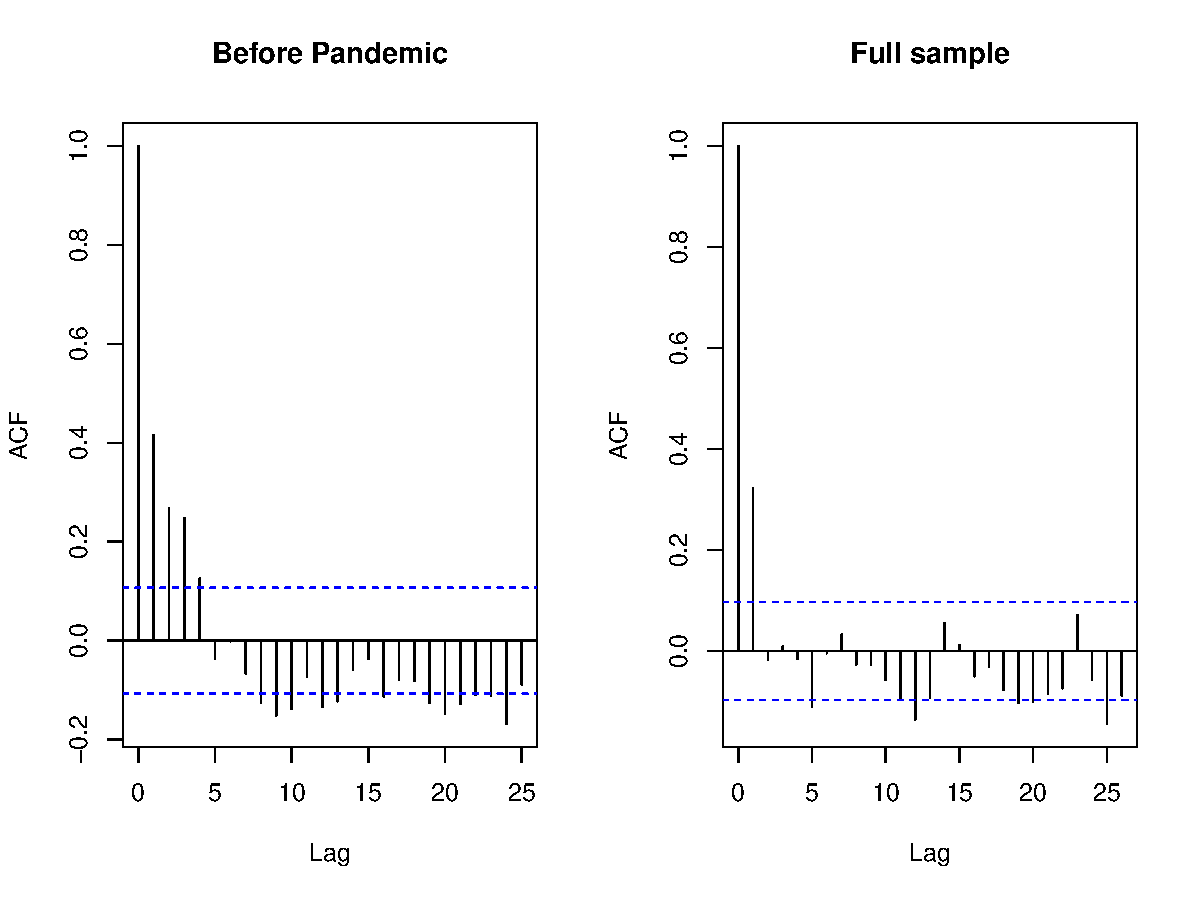
\includegraphics[height=3in, width=4in]{ACF_non_stat.pdf}\caption{Selected data: original (top left) and transformed (top right). Cross correlation functions (bottom) \label{cor}}\end{center}\end{figure}\end{frame}


\begin{frame} {Non-Stationarity/Structural Changes}
\begin{itemize}
\item Before Pandemic the data has a stronger and longer dependence (ARMA(model)): the data is \textbf{smoother}
\item On the \textbf{full} data set  the previous dependence structure simplifies to a simple lag-one dependence (MA(1)-model): the data is \textbf{noisier} (higher vola and more frequent zero-crossings)
\end{itemize}
\end{frame}









\section{Benchmarks and Direct AR Forecasts}

\frame{\sectionpage}

\subsection{Design}

\begin{frame} {Benchmarks and Direct AR Predictors}
\begin{itemize}
\item Use data from 1990-02-01 to 2025-02-01 
\begin{itemize}
\item Singular readings during pandemic affect OLS estimation
\item Use trimmed scaled data (threshold $\pm 5$)
\end{itemize}

\item Denote $target_{t}(h)$: first column of real-time data matrix, i.e. real-time $BIP$ shifted forward by lag+h=7
\begin{itemize}
\item Stair-step extrapolation not ideal  
\end{itemize}
\item Benchmark 1: mean of BIP, i.e., $\frac{1}{t}\sum_{k=1}^t BIP_k$
\item Benchmark 2: regression of target on BIP:
\[target_{t}(h)=c+a_1 BIP_{t}+...+a_pBIP_{t-p}+\epsilon_t\]
\item Additional benchmarks: regress any of the real-time indicators on target 
\end{itemize}
\end{frame}





\begin{frame} {ARMA-Models}
\begin{itemize}
\item For each transformed series we can fit an ARMA-model: $p=3$, $q=1$
\item The model is not used for direct forecasts (which are based on OLS regression, see previous slides) 
\item Instead, the ARMA-models are used for computing the real-time filters, see below
\item For each model we can obtain its MA-inversion, see next plot in the case of BIP
\end{itemize}
\end{frame}




\begin{frame} {Benchmark 2: ACF and MA-Inversion of BIP}
\begin{figure}[H]\begin{center}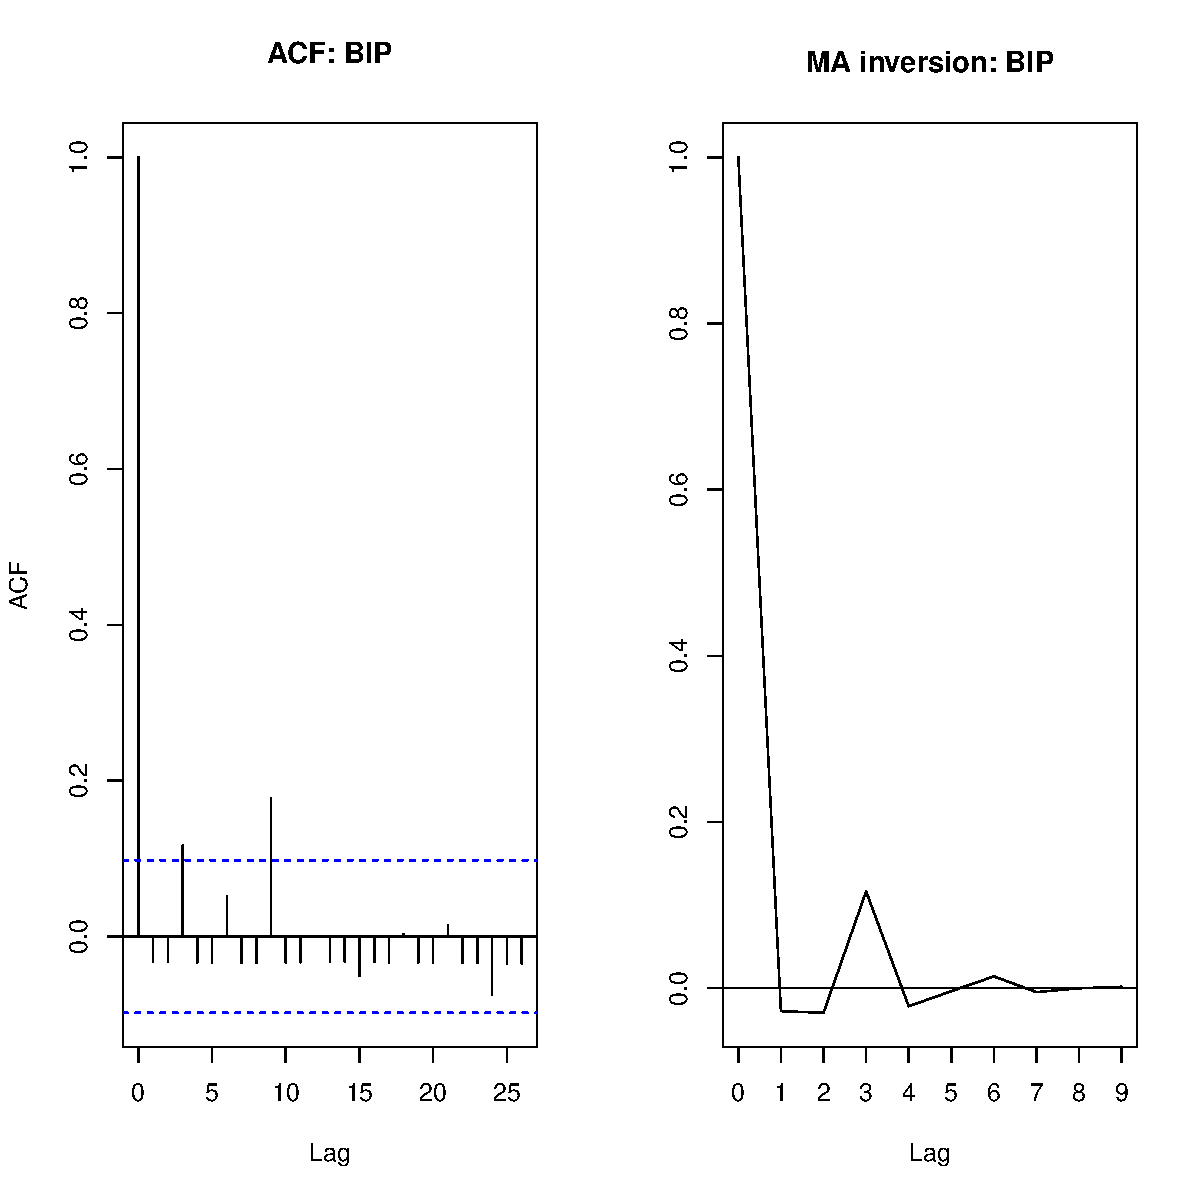
\includegraphics[height=3in, width=4.5in]{ma_inv_ip.pdf}\caption{\label{data}}\end{center}\end{figure}\end{frame}


\begin{frame} {Findings Benchmark 2}
\begin{itemize}
\item The MA-inversion of BIP as well as the ACF are close to white noise, i.e., \textbf{Benchmark 1$\approx$Benchmark 2}.
\begin{itemize}
\item Stair-step interpolation not ideal 
\item The regressors in the direct AR predictors are insignificant, see t-values further down
\item This result is reliant on the span for estimation (with/without Pandemic), see below for further details
\end{itemize}
\end{itemize}
\end{frame}


\begin{frame} {Forecast horizon}
\begin{itemize}
\item We here emphasize a one quarter ahead forecast horizon $h=3$
\item Alternative horizons such as $h=0$ or $h=12$ lead to similar qualitative outcomes but significance levels (t-tests) are affected
\end{itemize}
\end{frame}


\subsection{Performances}



\begin{frame} {Relative Forecast Performances}
\begin{itemize}

\item Regress the (real-time) indicator $y_{it}$ on the target to obtain the associated $MSE_i=E[\hat{\epsilon}_{it}^2]$, where $\hat{\epsilon}_{it}$ is the residual of the regression

\item Relative forecast MSEs: $MSE_i/MSE(benchmark)$. 
\item We can consider Benchmark 1 or 2 (mean of BIP or AR forecast based on BIP: virtually the same)
\item Numbers smaller one indicate outperformance of the corresponding indicator
\item The following table summarizes performances for the \textbf{entire} sample (pmi would be in the middle)
\end{itemize}

\end{frame}




\begin{frame} {Relative Forecast Performances: Forecast Benchmarks, $h=3$, Full Sample}\label{rmse1}

% latex table generated in R 4.2.2 by xtable 1.8-4 package
% Sat Feb 15 08:35:44 2025
\begin{table}[ht]
\centering
\begin{tabular}{rr}
  \hline
 & Relative MSE h=3 \\ 
  \hline
BIP & 1.00000 \\ 
  ip & 0.99472 \\ 
  ifo\_c & 1.00007 \\ 
  ifo\_exp & 1.00054 \\ 
  ifo\_l & 0.99378 \\ 
  ESI & 1.00078 \\ 
  spr\_10y\_3m & 0.99615 \\ 
   \hline
\end{tabular}
\caption{Relative mean-square performances against benchmark 2 (which is virtually identical with benchmark 1, the mean of BIP).} 
\label{perf_var1}
\end{table}\end{frame}

\subsection{Effect of Evaluation Sample}


\begin{frame} {Effect of Sample Selection}
\begin{itemize}
\item The above predictors and the evaluation span rely on the full sample, including Pandemic
\item All results are statistically insignificant, see below for details
\item What happens if we discard the singular (trimmed) Pandemic?
\item The following table reports relative MSEs for data prior to 2019-01-01 
\end{itemize}

\end{frame}



\begin{frame} {Relative Forecast Performances: Evaluation on Data Before Pandemic}\label{rmse2}

% latex table generated in R 4.2.2 by xtable 1.8-4 package
% Sat Feb 15 08:35:44 2025
\begin{table}[ht]
\centering
\begin{tabular}{rr}
  \hline
 & Relative MSE h=3 \\ 
  \hline
BIP & 1.00000 \\ 
  ip & 0.99895 \\ 
  ifo\_c & 0.96738 \\ 
  ifo\_exp & 0.97755 \\ 
  ifo\_l & 0.97750 \\ 
  ESI & 0.98354 \\ 
  spr\_10y\_3m & 0.99520 \\ 
   \hline
\end{tabular}
\caption{Relative mean-square performances against benchmark 2 (which is virtually identical with benchmark 1, the mean of BIP).} 
\label{perf_var1}
\end{table}\end{frame}




\begin{frame} {Findings}
\begin{itemize}
\item Indicators perform less well \textbf{after} 2019-01-01 in relative terms
\item Ifo series perform best (before Pandemic)
\item Difference is statistically significant (see below for more detailed results)
\end{itemize}

\end{frame}


\section{Univariate Filters}

\frame{\sectionpage}


\subsection{Alternative Targets}


\begin{frame} {Alternative Targets}
\begin{itemize}
\item Instead of looking at BIP-returns shifted by $lag+h$ (7-steps ahead) we might be interested in looking at the \textbf{trend} of BIP-returns: \emph{trend-growth}
\item Which `trend'?
\begin{itemize}
\item Ideal trend, model-based trend (SEATS, state-space), Henderson, Hodrick Prescott (HP),...
\end{itemize}
\item Due to its wide use in applications we look at \textbf{HP}(14400) (monthly design)
\item On the next slide, we plot and compare the two targets: original shifted BIP (violet line) and HP applied to shifted BIP (brown)
\end{itemize}
\end{frame}




\begin{frame} {Targets 1 and 2: BIP-Shifted (violet), BIP-Trend (brown), ip Real-Time (black): All Series Standardized }
\begin{figure}[H]\begin{center}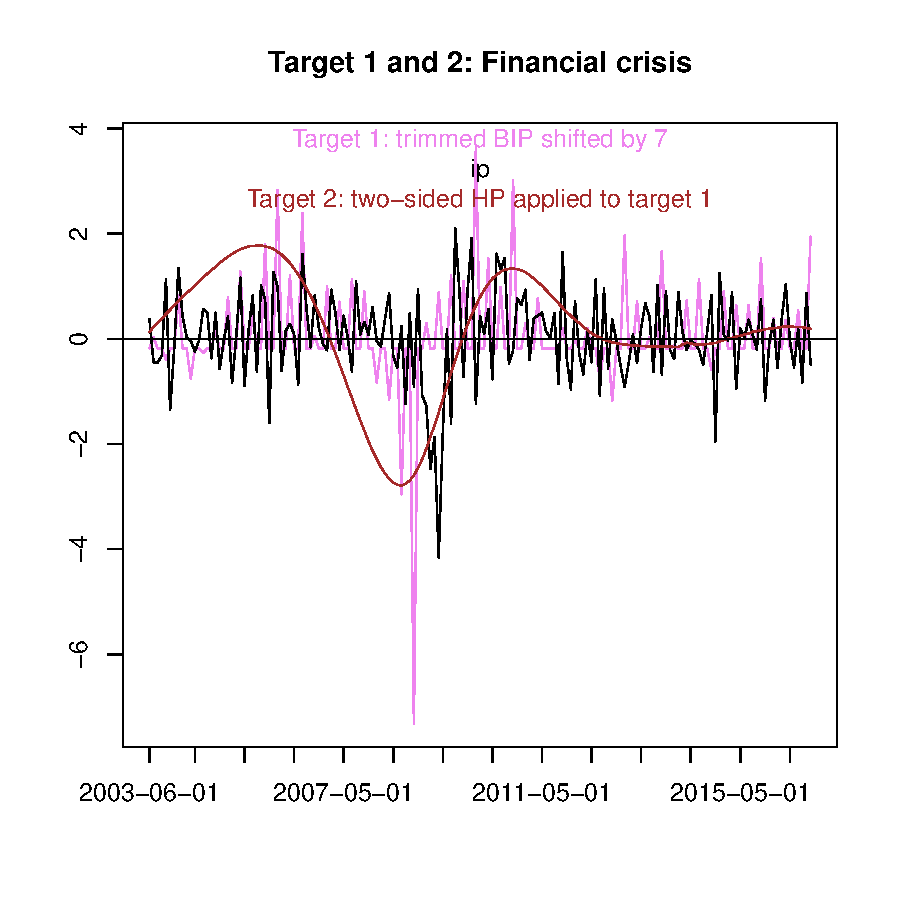
\includegraphics[height=3in, width=4.5in]{alternative_targets_1.pdf}\caption{\label{data}}\end{center}\end{figure}\end{frame}





\begin{frame} {Findings}
\begin{itemize}
\item The filter output (target 2: brown) tracks the (long-term/systematic) trend-growth of target 1 (violet)
\begin{itemize}
\item Business-cycle or \textbf{growth-cycle}: depending on how the filter is implemented, a negative sign can be associated with negative economic growth (growth cycle), under-par growth (below potential output), recessions/crises (see SSA paper)
\item The sign of the filtered data, i.e., its \emph{zero-crossings}, have a potentially meaningful \emph{economic} interpretation
\end{itemize}
\item \textbf{Problem}: two-sided (acausal) filter cannot be computed in real-time 
\end{itemize}
\end{frame}






\subsection{Causal Filter Design}

\begin{frame} {Causal Filter Design}
\begin{itemize}
\item We can apply the two-sided HP to each indicator (ip, ifo, ESI, spread,...)
\item \textbf{Task}: for each indicator compute a \emph{causal} filter which tracks the two-sided HP (applied to that indicator) 
\begin{itemize}
\item \textbf{MSE} and \textbf{SSA} designs: the latter encompasses the former (see SSA paper)
\item We account for $h$ and the publication lag of each indicator (details left aside)
\end{itemize}
\item New \textbf{predictors}: MSE and SSA (applied to indicators)
\item Potentially interesting \textbf{targets}
\begin{itemize}
\item We here continue to look at \emph{BIP-shifted} (violet line in above plot) as our main target of interest 
\item Later, we also consider \emph{BIP-trend}, i.e. the two-sided HP  applied to BIP-shifted (brown line), as an alternative target
\end{itemize}
\end{itemize}
\end{frame}





\begin{frame} {Forecast Performance}\label{overf}
\begin{itemize}
\item For each indicator, we compute the mean-square forecast error $E[(BIP_{t+h}-\hat{T}_{ti})^2]$, where $BIP_{t+h}$ is the target series (shifted BIP) and $\hat{T}_{ti}$ is either the MSE- or the SSA-output when applied to  the $i-$th indicator
\item Note that by design, $\hat{T}_{ti}$ does not target $BIP_{t+h}$. Instead it tracks the two-sided HP applied to the $i$-th indicator (accounting for $h$ and publication lag of that indicator) 
\item \textbf{Idea}: if $\hat{T}_{ti}$ tracks the (future) trend-growth of the $i$-th indicator and if the indicator is informative about the effective target $BIP_{t+h}$, then $\hat{T}_{ti}$ should also track $BIP_{t+h}$ `somehow'
\begin{itemize}
\item Validate MSE- and SSA-trends by computing performances against the `indirect' target $BIP_{t+h}$ 
\end{itemize}
\end{itemize}
\end{frame}

\begin{frame} {MSE and SSA for BIP}
\begin{itemize}
\item The figure on the next slide displays
\begin{itemize}
\item The \textbf{MA inversion} of the ARMA-model fitted to BIP (top left)
\item The \textbf{acausal} two-sided HP (top right)
\item The \textbf{causal} filters: MSE (green), SSA (blue) and classic concurrent HP-C (violet)
\end{itemize}
\end{itemize}
\end{frame}




\begin{frame} {Univariate Filters for BIP}
\begin{figure}[H]\begin{center}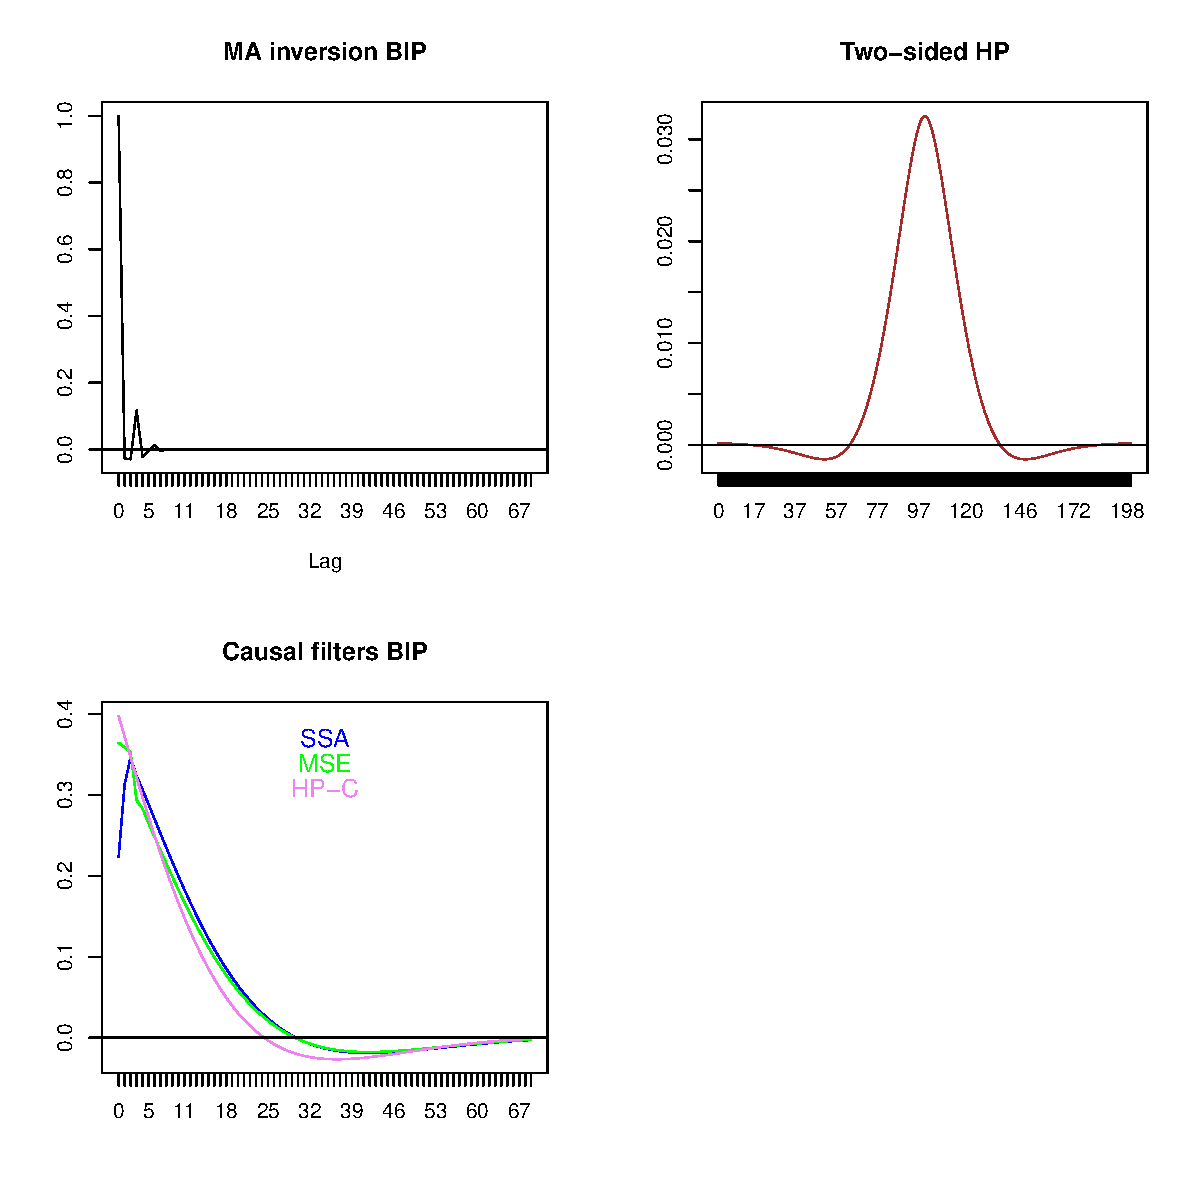
\includegraphics[height=3in, width=4.5in]{filt_coef_INDPRO_uni_x.pdf}\caption{\label{data}}\end{center}\end{figure}\end{frame}



\subsection{Performances: Comparison with AR-Benchmarks}


\begin{frame} {Relative Forecast Performances}
\begin{itemize}
\item In the next table, we compare relative forecast performances of all predictors
\begin{itemize}
\item direct \textbf{AR} forecasts based on indicators: first column
\item trend forecasts \textbf{SSA}: second column
\item trend forecasts \textbf{MSE}: third column
\end{itemize}
\item Relative forecast error: all forecast mean-square errors are normalized by AR-forecast based on BIP (benchmark 2). 
\begin{itemize}
\item Numbers smaller one signify outperformance of the benchmark (significance is analyzed further down)
\end{itemize}
\item We assume \textbf{calibrated} filters, i.e., we regress filters on target to account for (static) level and scale parameters (filters implicitly assume the data to be centered and the scale differs from BIP) 
\end{itemize}
\end{frame}

\begin{frame} {Relative Forecast Performances: $h=3$ Full Sample}\label{rmse3}

% latex table generated in R 4.2.2 by xtable 1.8-4 package
% Sat Feb 15 08:35:44 2025
\begin{table}[ht]
\centering
\begin{tabular}{rrrr}
  \hline
 & Direct AR forecasts & SSA & MSE \\ 
  \hline
BIP & 1.0000 & 1.0048 & 1.0053 \\ 
  ip & 0.9947 & 1.0066 & 1.0069 \\ 
  ifo\_c & 1.0001 & 0.9897 & 0.9908 \\ 
  ifo\_exp & 1.0005 & 0.9859 & 0.9888 \\ 
  ifo\_l & 0.9938 & 0.9947 & 0.9941 \\ 
  ESI & 1.0008 & 0.9924 & 0.9945 \\ 
  spr\_10y\_3m & 0.9961 & 0.9937 & 0.9931 \\ 
   \hline
\end{tabular}
\caption{Relative mean-square performances against benchmark 2 (which is virtually identical with benchmark 1, the mean of BIP).} 
\label{perf_var1}
\end{table}\end{frame}






%\begin{frame} {Relative Forecast Performances: `Regression'}

%<<label=ats_mba_2,echo=FALSE,results=tex>>=

%mat<-lm_perf_mat
%xtable((mat), dec = 1,digits=rep(2,dim(mat)[2]+1),
%paste("Relative mean-square performances against benchmark 2 (which is virtually identical with benchmark 1, the mean of ip)."),
%label=paste("perf_var1",sep=""),
%center = "centering", file = "", floating = FALSE)
%@
%\end{frame}




\begin{frame} {Discussion}
\begin{itemize}
\item Calibrated trend forecasts (second and third columns) are generally not worse than `direct' AR indicator forecasts (first column)
\item MSE and SSA are similar (the latter is smoother: less zero-crossings, see below for details)

\item \textbf{Significance}: t-values in regressions of predictors on target, see next slide

\end{itemize}

\end{frame}



\begin{frame} {Significance ($h=3$)}\label{tstat1}


% latex table generated in R 4.2.2 by xtable 1.8-4 package
% Sat Feb 15 08:35:44 2025
\begin{table}[ht]
\centering
\begin{tabular}{rrrr}
  \hline
 & t\_stat direct AR & t-stat SSA & t-stat MSE \\ 
  \hline
BIP & 0.44 & -0.79 & -0.70 \\ 
  ip & 1.40 & -0.31 & -0.08 \\ 
  ifo\_c & 0.40 & 2.30 & 2.22 \\ 
  ifo\_exp & 0.13 & 2.54 & 2.35 \\ 
  ifo\_l & 1.46 & 1.93 & 1.98 \\ 
  ESI & -0.18 & 2.11 & 1.95 \\ 
  spr\_10y\_3m & 1.25 & 2.00 & 2.06 \\ 
  Consensus & 2.11 & 2.51 & 2.48 \\ 
   \hline
\end{tabular}
\caption{Significance of predictors: t-statistics from a regression of the predictors on the target. Consensus forecast is the equally weighted mean of all forecasts.} 
\label{perf_var1}
\end{table}\end{frame}


\begin{frame} {Findings}
\begin{itemize}
\item Direct AR predictors are insignificant (on full sample, including Pandemic)
\item SSA and MSE similar (with respect to t-statistics) and some of them are significant
\item \textbf{Consensus} (equally-weighted) generally perform well
\end{itemize}
\end{frame}







\subsection{Effect of Evaluation Sample}


\begin{frame} {Relative Forecast Performances: Evaluation on Data Before Pandemic}\label{rmse4}

% latex table generated in R 4.2.2 by xtable 1.8-4 package
% Sat Feb 15 08:35:44 2025
\begin{table}[ht]
\centering
\begin{tabular}{rrrr}
  \hline
 & Direct AR forecasts & SSA & MSE \\ 
  \hline
BIP & 1.00 & 1.00 & 1.00 \\ 
  ip & 1.00 & 1.01 & 1.01 \\ 
  ifo\_c & 0.97 & 0.98 & 0.97 \\ 
  ifo\_exp & 0.98 & 0.96 & 0.96 \\ 
  ifo\_l & 0.98 & 1.00 & 0.99 \\ 
  ESI & 0.98 & 0.98 & 0.98 \\ 
  spr\_10y\_3m & 1.00 & 0.99 & 0.99 \\ 
   \hline
\end{tabular}
\caption{Relative mean-square performances against benchmark 2: data prior to Pandemic.} 
\label{perf_var1}
\end{table}\end{frame}



\begin{frame} {Significance: Data prior to Pandemic}\label{tstat2}

% latex table generated in R 4.2.2 by xtable 1.8-4 package
% Sat Feb 15 08:35:44 2025
\begin{table}[ht]
\centering
\begin{tabular}{rrrr}
  \hline
 & t\_stat direct AR & t-stat SSA & t-stat MSE \\ 
  \hline
BIP & 0.81 & -1.41 & -1.37 \\ 
  ip & 1.12 & -1.21 & -0.96 \\ 
  ifo\_c & 2.98 & 2.62 & 2.96 \\ 
  ifo\_exp & 2.49 & 3.35 & 3.67 \\ 
  ifo\_l & 2.52 & 1.72 & 1.98 \\ 
  ESI & 2.13 & 2.68 & 2.86 \\ 
  spr\_10y\_3m & 1.50 & 2.24 & 2.32 \\ 
  Consensus & 3.25 & 2.82 & 3.14 \\ 
   \hline
\end{tabular}
\caption{Significance of predictors: t-statistics from a regression of the predictors on the target. Consensus forecast is the equally weighted mean of all forecasts.} 
\label{perf_var1}
\end{table}\end{frame}



\begin{frame} {Findings}
\begin{itemize}
\item \textbf{Main effect}: t-statistics \textbf{markedly larger} (despite shorter sub-span)
\item Direct AR forecasts often strongly significant: performances similar to filters
%\item Ranking (hierarchy) of direct AR-forecasts \textbf{affected}: ifo-exp and ifo-c are more important than ESI on shorter sub-sample 
%\item Hierarchy of trend forecasts less affected 

\end{itemize}
\end{frame}



\begin{frame} {Alternative Evaluation Criteria}
\begin{itemize}
\item Until yet we emphasized the mean-square forecast error
\item Question: what about \textbf{smoothness}, i.e., noise suppression and reliability? 
\begin{itemize}
\item Original justification for trend targets: for identical (relative) forecast performances we might prefer a \textbf{more reliable/regular} (smoother/less noisy) forecast rule
\item The above results suggest that MSE forecast performances are \textbf{not} negatively affected by filtering (`trends')
\item What about \textbf{zero-crossings} and shape/dynamics of filter outputs vs. direct AR forecasts
\item And what about \textbf{retardation} (lag/right-shift) of trend forecasts?
\end{itemize}
\end{itemize}
\end{frame}



\subsection{Zero-Crossings and Holding Time}


\begin{frame} {Zero-Crossings and Holding Times}\label{htzc1}
\begin{itemize}
\item \textbf{Holding time} (HT): mean duration between consecutive zero-crossings
\item \textbf{SSA}: impose $50\%$ larger \emph{expected }HT than MSE 
\begin{itemize}
\item Dual formulation of SSA \textbf{optimization} principle: \emph{maximize HT} for given tracking accuracy (target correlation or MSE)
\end{itemize}
\item Compute and compare \emph{empirical} HTs (larger = smoother):
\end{itemize}

% latex table generated in R 4.2.2 by xtable 1.8-4 package
% Sat Feb 15 08:35:44 2025
\begin{table}[ht]
\centering
\begin{tabular}{rrrr}
  \hline
 & HT AR & HT MSE & HT SSA \\ 
  \hline
BIP & 2.27 & 19.00 & 23.38 \\ 
  ip & 1.68 & 7.07 & 11.26 \\ 
  ifo\_c & 3.01 & 11.26 & 14.48 \\ 
  ifo\_exp & 2.95 & 9.81 & 11.69 \\ 
  ifo\_l & 2.69 & 9.81 & 16.00 \\ 
  ESI & 2.64 & 12.67 & 19.00 \\ 
  spr\_10y\_3m & 2.81 & 9.50 & 12.67 \\ 
   \hline
\end{tabular}
\caption{Empirical (sample) Holding times of predictors: direct AR, MSE and SSA.} 
\label{perf_var1}
\end{table}\end{frame}



\begin{frame} {Zero-Crossings and Holding Times}
\begin{itemize}
\item Filters much smoother (less crossings) than direct AR forecasts
\item Sample HTs of M-SSA approximately 50$\%$ larger than MSE (series are centered and therefore expected and sample HTs match better than in ip-case: see corresponding slides)
\item On the folowing slide we display AR-forecasts (orange) and MSE- (green) and SSA-filters (blue) 
\begin{itemize}
\item Zero-crossings are marked by corresponding colored vertical lines
\item Series are standardized (scaled and centered)
\end{itemize}
\end{itemize}
\end{frame}


%\begin{frame} {Zero-crossings ifo-exp: post Financial Crisis}
%<<label=z_box_plot_pure_mba_2.pdf,echo=FALSE,results=tex>>=
%file = "zero_cross_ifo_exp.pdf"
%cat("\\begin{figure}[H]")
%cat("\\begin{center}")
%cat("\\includegraphics[height=3in, width=4.5in]{", file, "}\n",sep = "")
%cat("\\caption{", sep = "")
%cat("\\label{data}}", sep = "")
%cat("\\end{center}")
%cat("\\end{figure}")
%@
%\end{frame}


\begin{frame} {Zero-crossings BIP: Standardized Series}
\begin{figure}[H]\begin{center}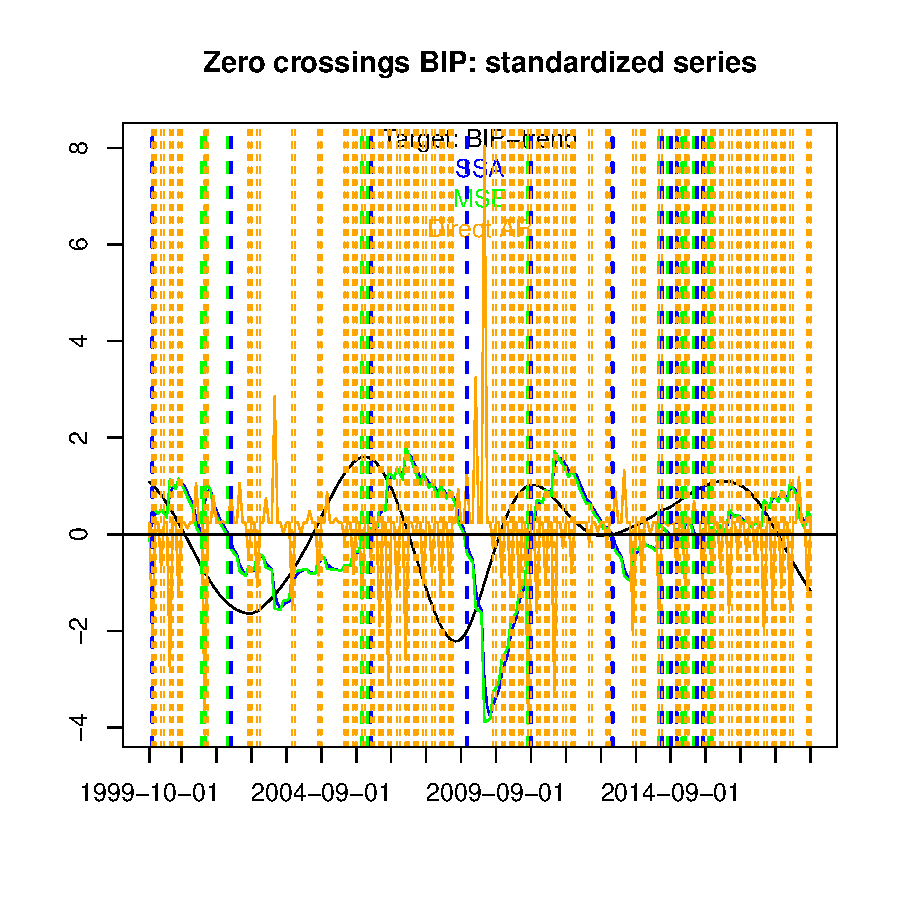
\includegraphics[height=3in, width=4.5in]{zero_cross_ifo_l_1.pdf}\caption{\label{data}}\end{center}\end{figure}\end{frame}



\begin{frame} {Findings}
\begin{itemize}
\item See similar comments in ip-case (slides ip)
\item Sign of lagged BIP is negative (predictor is not significant): explains `strange' readings of direct AR predictor (orange) during financial crisis
\end{itemize}
\end{frame}







\section{Multivariate Filters}

\frame{\sectionpage}












\subsection{Dependence}


\begin{frame} {Dependence}
\begin{itemize}
\item Multivariate M-MSE and M-SSA: rely on several time series to track the two-sided HP 
\item For the multivariate design we consider BIP, ip, ifo-exp, ESI, spr-10y-3m
\begin{itemize}
\item Criterion for \textbf{selection}: the above series differ in terms of leads/lags (see CCF on slide \eqref{ccf}) \item Therefore a multivariate design can exploit  the mutually differing (as well as the common) features of each series (see below) 
\end{itemize}
\item The next two slides display the \textbf{CCF}s corresponding to the full sample (first slide) and data up to the Pandemic (second slide) 
\begin{itemize}
\item The CCF refers to the \emph{real-time} data: after accounting for publication lags
\end{itemize}
\end{itemize}

\end{frame}


\begin{frame} {CCF: Full Data Set}\label{ccf_pand_multe}
\begin{figure}[H]\begin{center}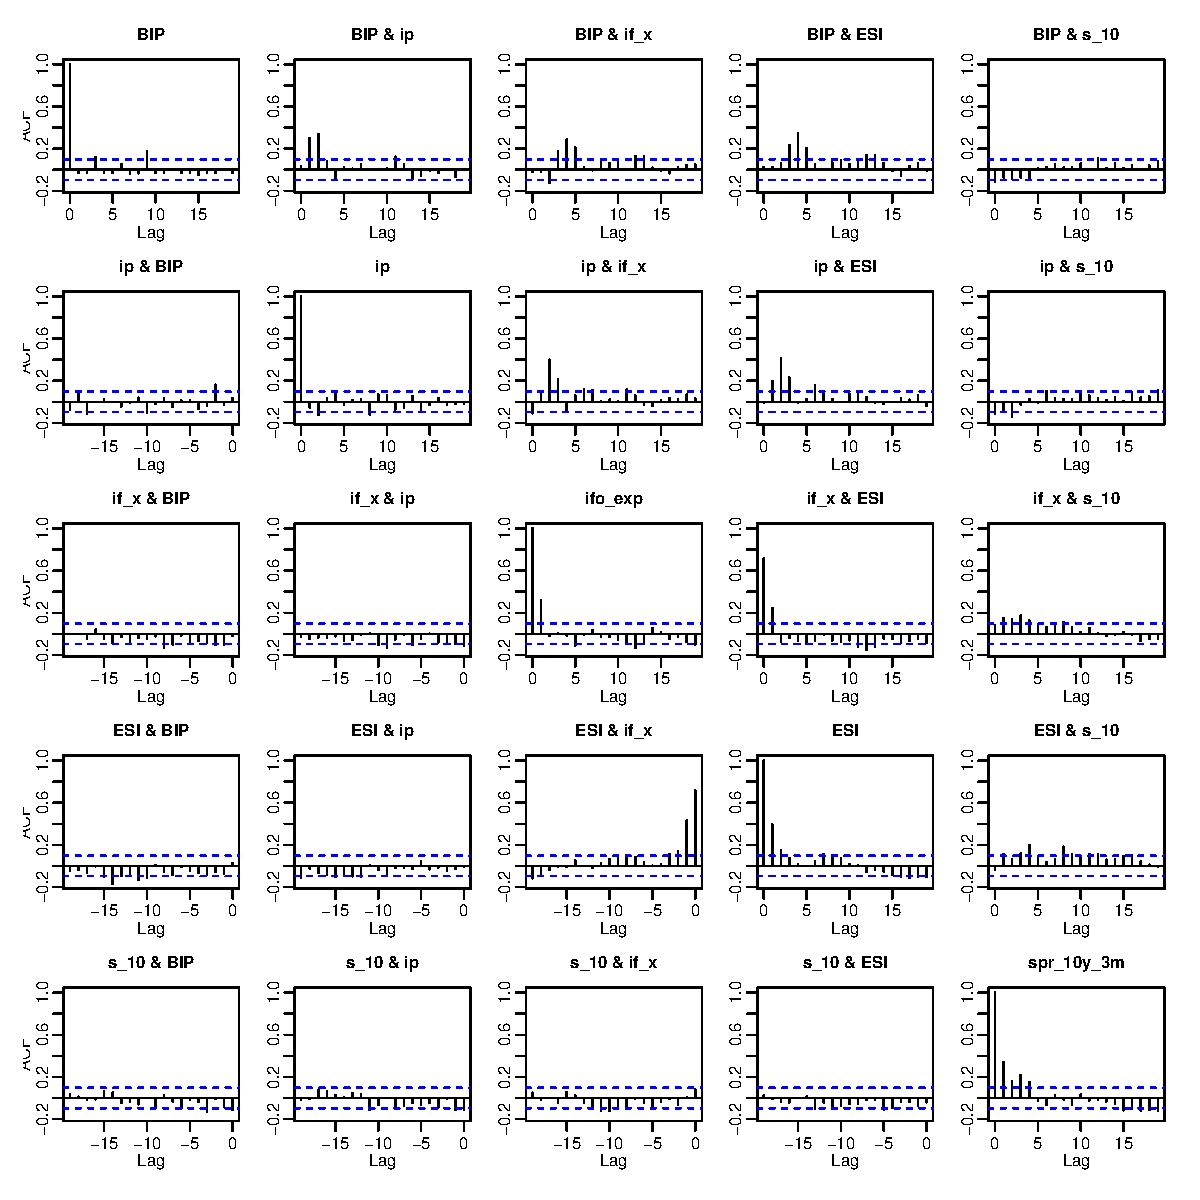
\includegraphics[height=3in, width=4in]{acf_all.pdf}\caption{MA-inversion of VARMA\label{cor}}\end{center}\end{figure}\end{frame}


\begin{frame} {CCF: Up to Pandemic}\label{ccf_pand_mult}
\begin{figure}[H]\begin{center}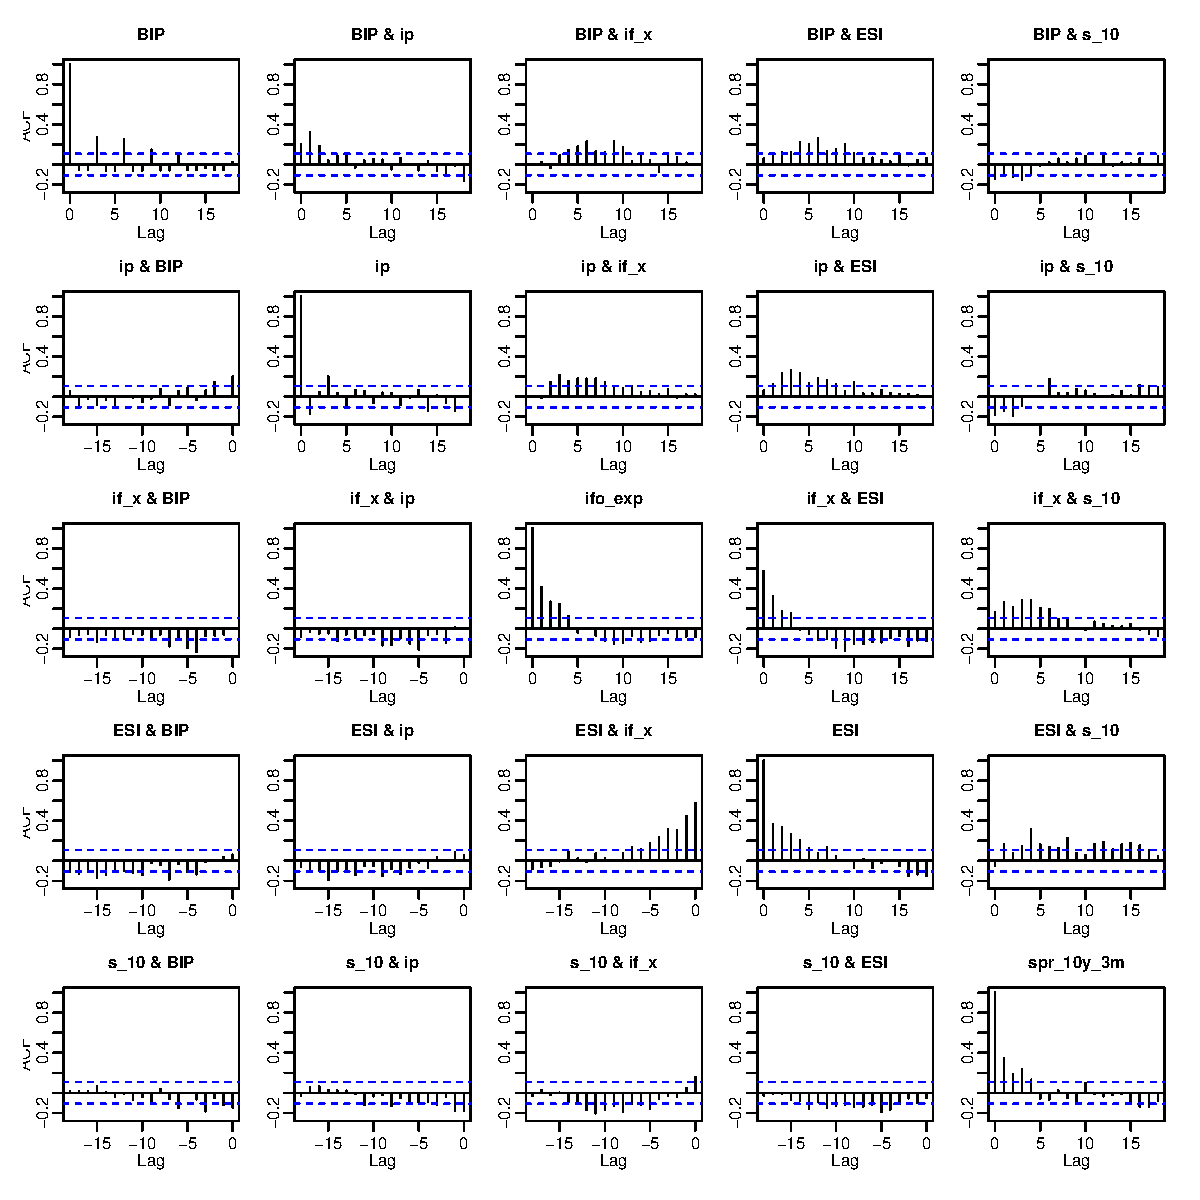
\includegraphics[height=3in, width=4in]{acf_pan.pdf}\caption{MA-inversion of VARMA\label{cor}}\end{center}\end{figure}\end{frame}

\begin{frame} {Findings}\label{slide_findings_ccf_mult}
\begin{itemize}
\item Significant ACFs of BIP at multiples of three months: effect of \textbf{stair-step} interpolation
\item \textbf{Non-stationarity}: dependence structure changes after pandemic (structural change?)
\item Dependence: BIP cross-correlates with ip, ifo and ESI (first row in above plots). 
\item Leads/lags correspond to peak-CCF on slide \eqref{ccf} (cross-check)
\item Additional findings: 
\begin{itemize}
\item \textbf{BIP} and \textbf{spread} are nearly \textbf{uncorrelated}! (at observed leads/lags) 
\item \textbf{Spread} seems to correlate with (and to lead) \textbf{ifo}-series (but not ip). Maybe spread enters somehow into construction of ifo?
\end{itemize}
\end{itemize}

\end{frame}




\subsection{VARMA}

\begin{frame} {VARMA}
\begin{itemize}
\item Fit a VARMA model to BIP, ip, ifo-exp, ESI, spr-10y-3m
\begin{itemize}
\item Rely on R-package MTS by Ruey Tsay (we also adopt regularization to avoid overfitting)
\end{itemize}
\item Purpose: VARMA model is used for M-SSA and M-MSE (need to account for leads/lags and CCF)
\item Estimation span: from first observation to $2024-11-01$
%\item Explanatories: BIP, ip, ifo-exp, ESI, spr-10y-3m 
\item Model orders: VARMA(2,0), see below for details 
\item The (V)MA-inversion of the VARMA is displayed on the next slide
\end{itemize}

\end{frame}


\begin{frame} {MA Inversion of VARMA}
\begin{figure}[H]\begin{center}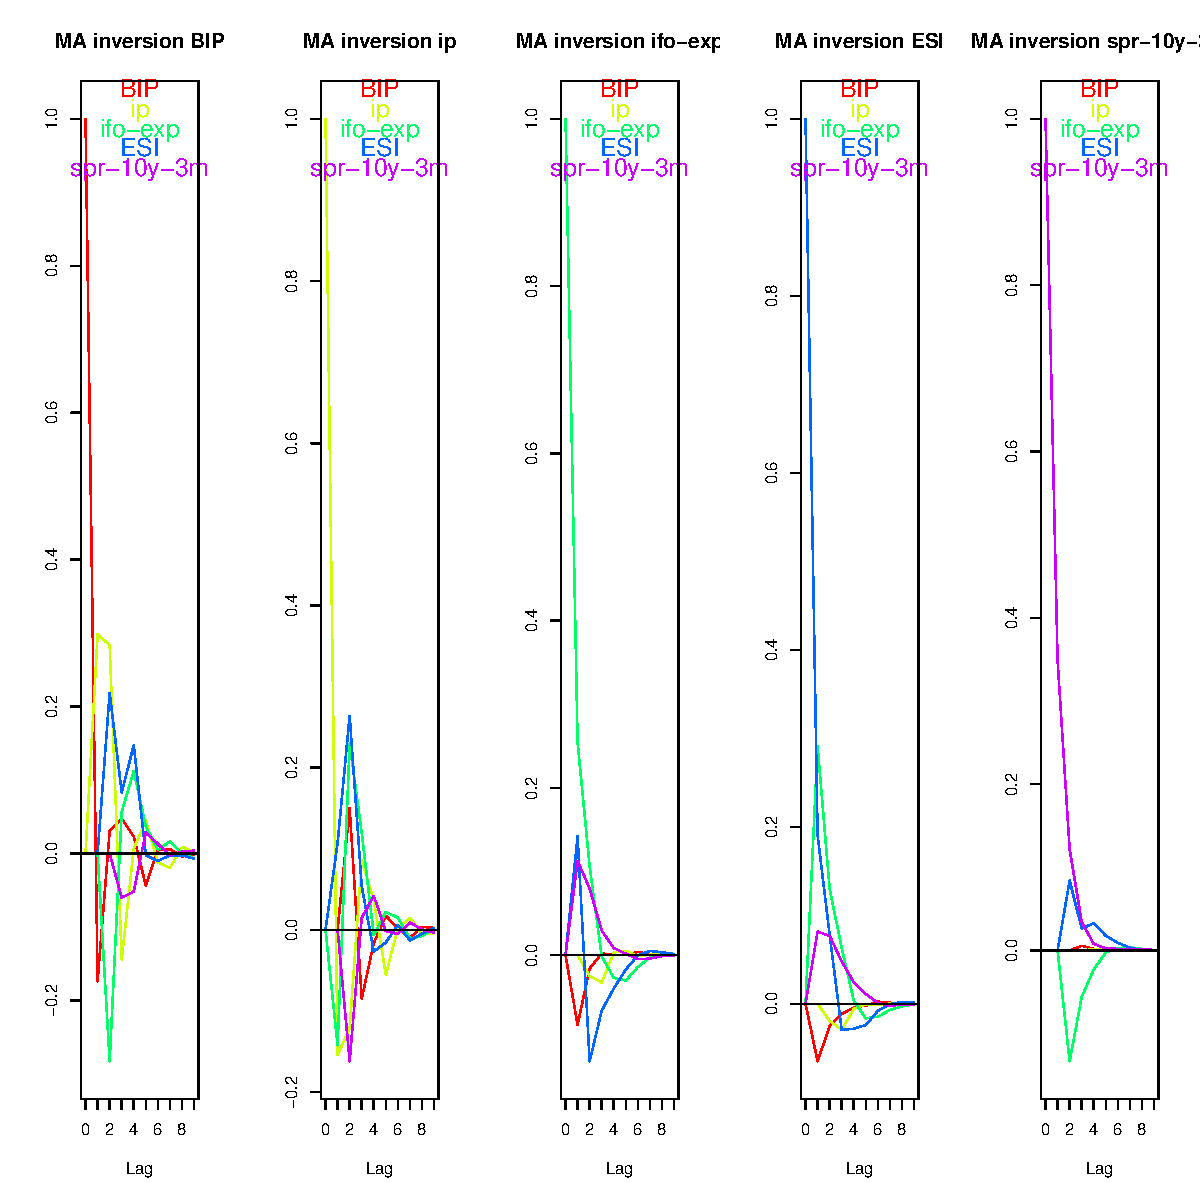
\includegraphics[height=3in, width=4in]{ma_inv_multi_ip.pdf}\caption{MA-inversion of VARMA\label{cor}}\end{center}\end{figure}\end{frame}


\begin{frame} {Findings}
\begin{itemize}
\item Interpretation: see ip-case (slides ip)
\item We can \textbf{interpret} VARMA model: simple and explainable
\end{itemize}

\end{frame}




\subsection{M-SSA and M-MSE Filter Design}

\begin{frame} {M-SSA and M-MSE Filters}
\begin{itemize}
\item For each series $y_{it}$, $i=1,...,5$ of the multivariate filter, the \textbf{target} $T_{it}$ is specified by applying the acausal HP to $y_{it}$ 
\begin{itemize}
\item \textbf{Same trend} targets as in univariate case 
\item But each trend target can rely on \emph{multiple} time series for deriving the \emph{causal} filter
\item \emph{VARMA}-model is used for computing the \emph{causal} filters
\end{itemize}
\item M-SSA: impose the \textbf{same HT} as in univariate case
\item Overall design decisions: compare \textbf{apples with apples} (can compare uni- and multivariate designs in a consistent way)
\item The following two slides display multivariate MSE (M-MSE) and SSA (M-SSA) filters
\end{itemize}

\end{frame}



\begin{frame} {M-MSE}\label{m_mse_p}
\begin{figure}[H]\begin{center}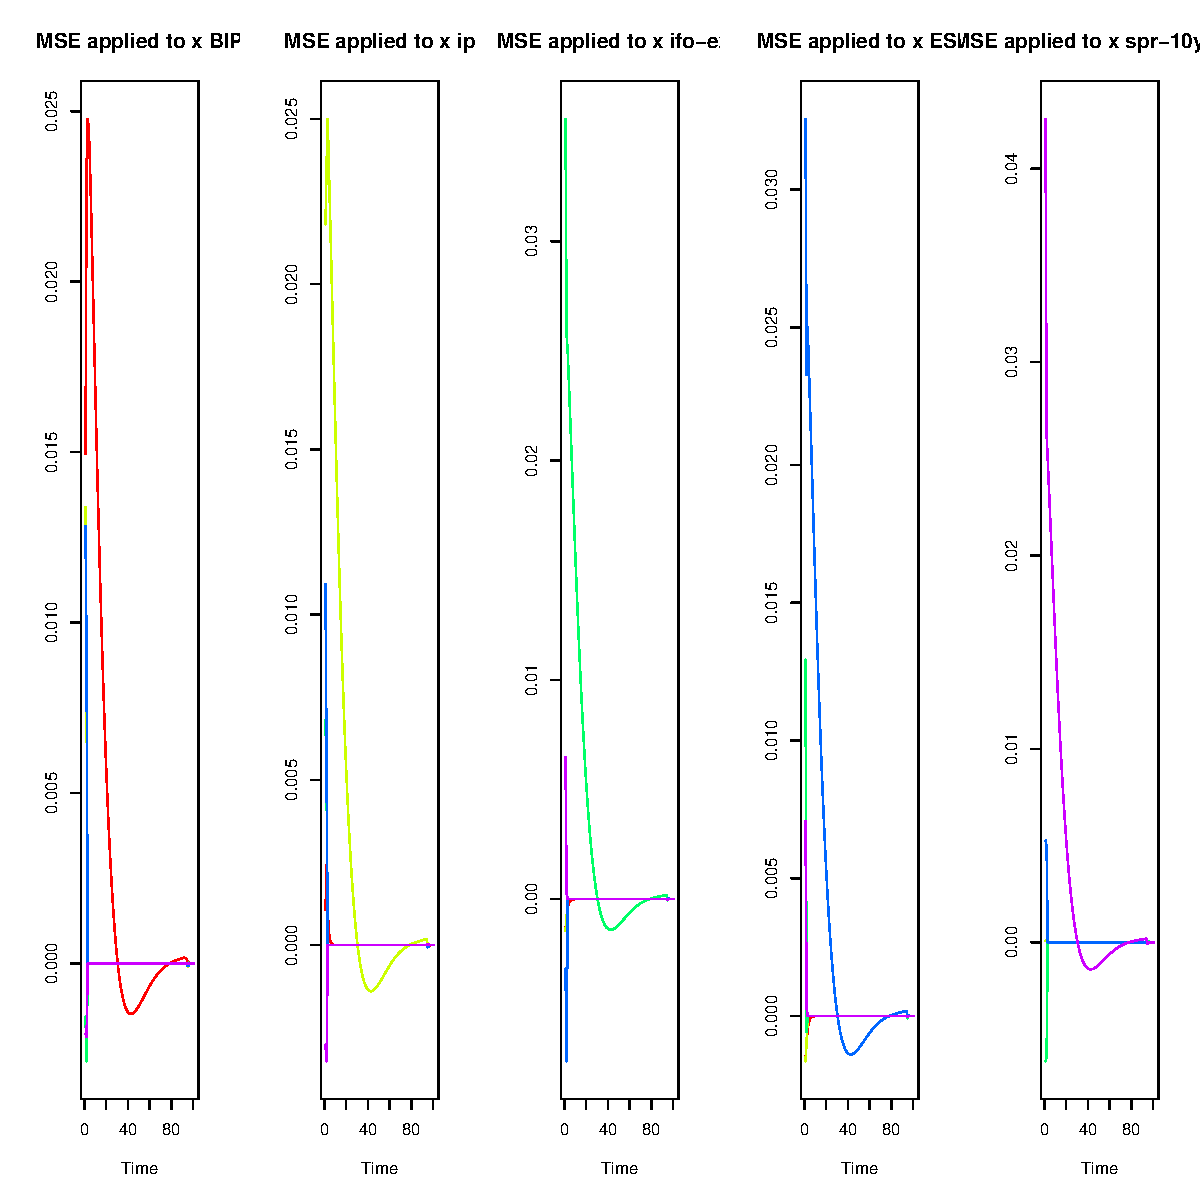
\includegraphics[height=3in, width=4in]{MSE_multi_ip.pdf}\caption{MA-inversion of VARMA\label{cor}}\end{center}\end{figure}\end{frame}

\begin{frame} {M-SSA}\label{m_ssa_p}
\begin{figure}[H]\begin{center}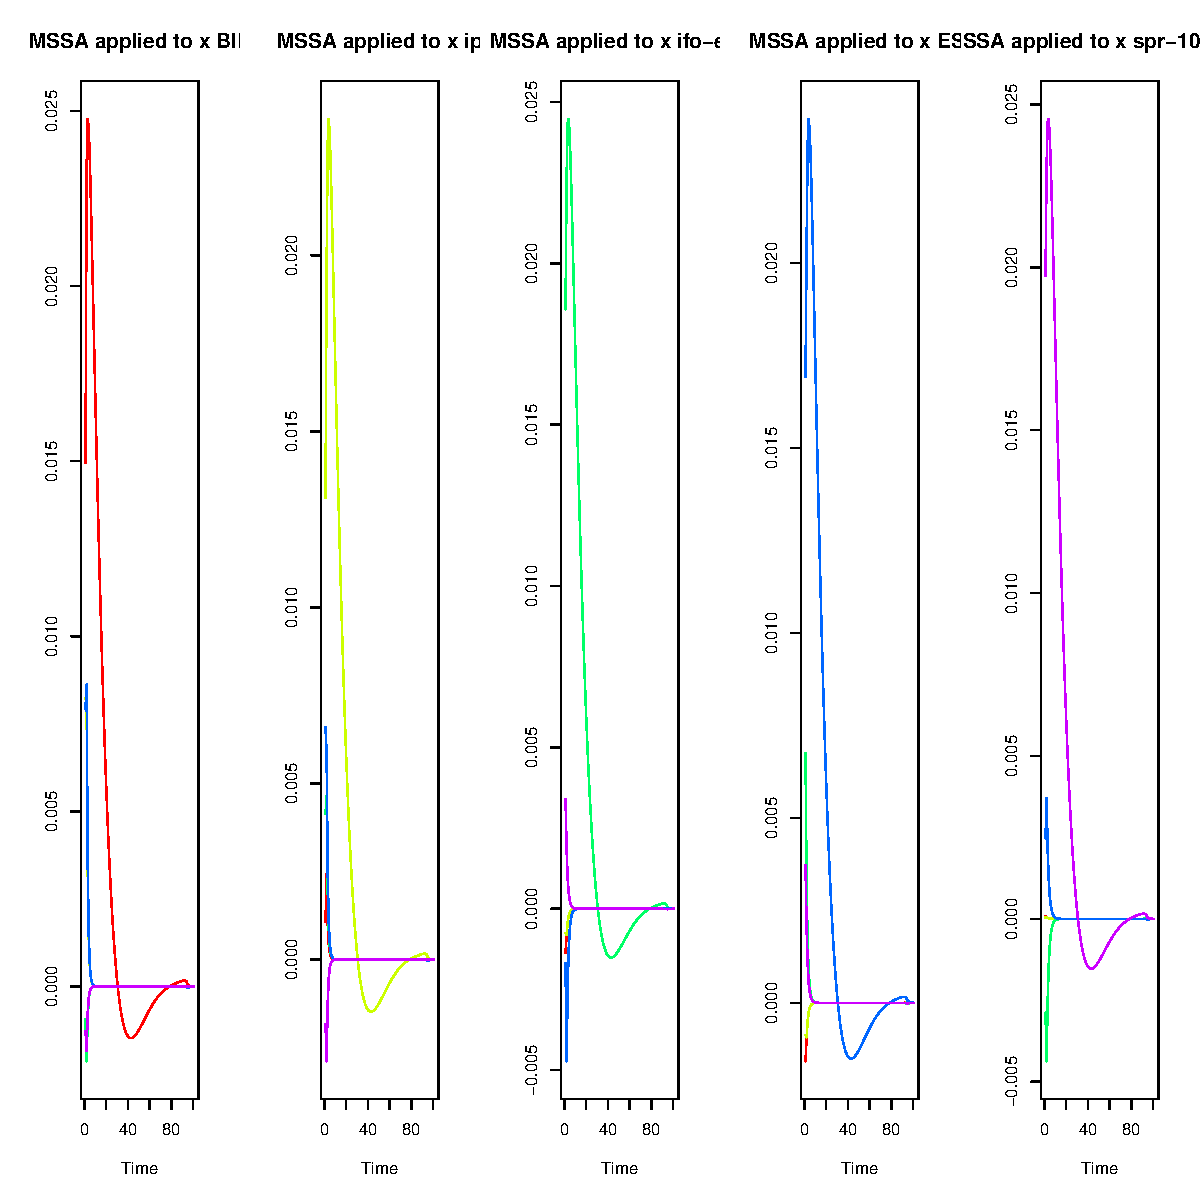
\includegraphics[height=3in, width=4in]{MSSA_multi_ip.pdf}\caption{MA-inversion of VARMA\label{cor}}\end{center}\end{figure}\end{frame}


\begin{frame} {MA-Inversion M-SSA: Filter as Applied to VARMA-Residuals}
\begin{figure}[H]\begin{center}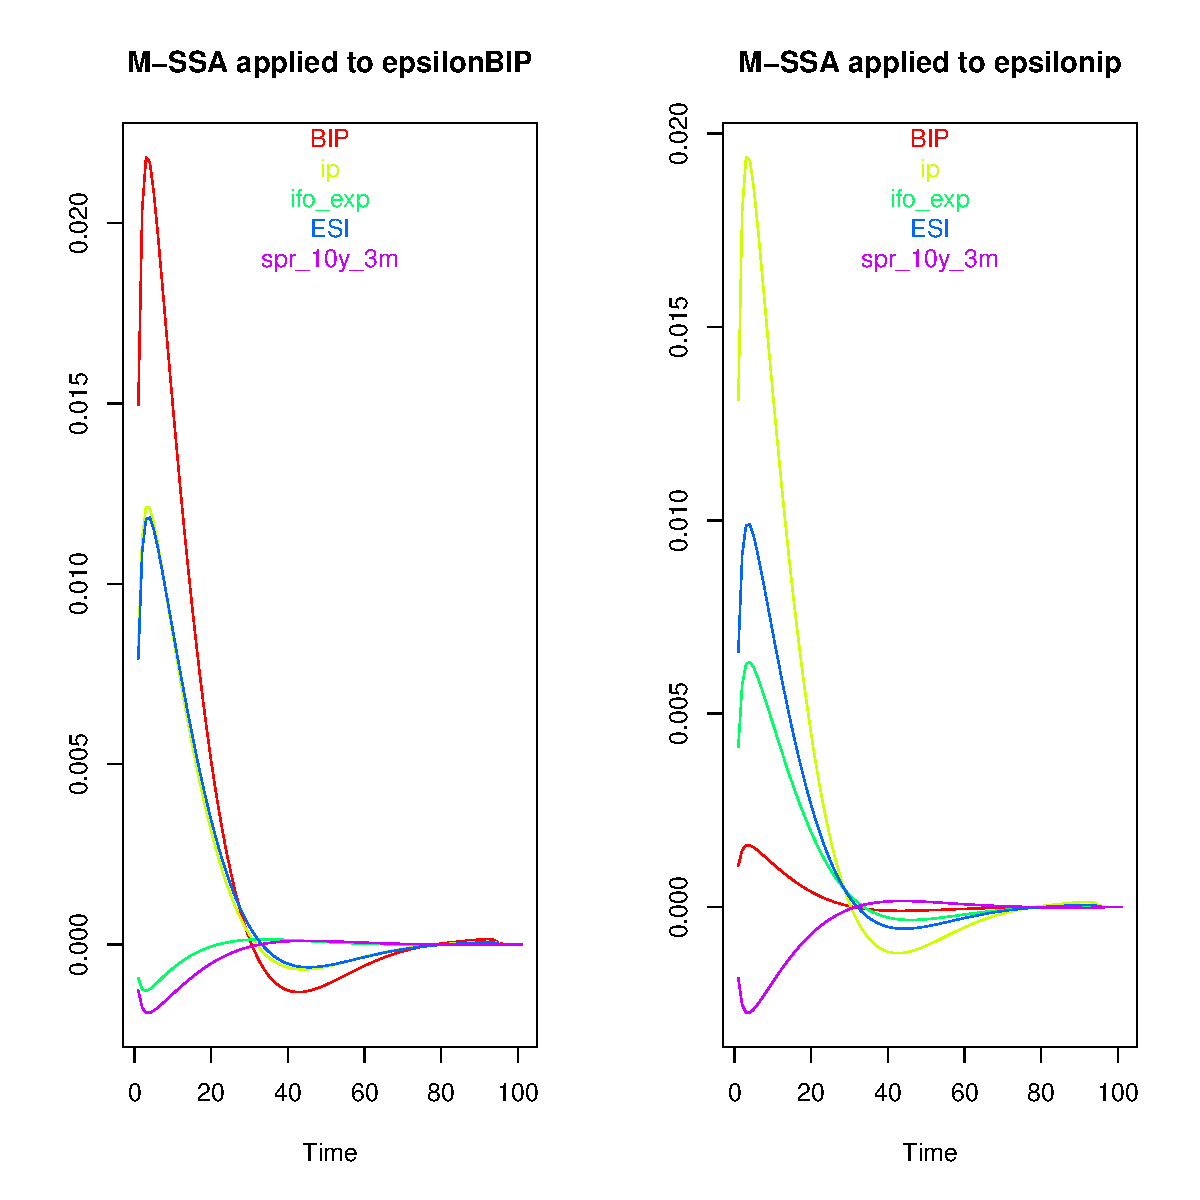
\includegraphics[height=3in, width=4in]{MSSA_multi_eps_ip.pdf}\caption{MA-inversion of VARMA\label{cor}}\end{center}\end{figure}\end{frame}



\begin{frame} {Findings}
\begin{itemize}
\item Interpretation: see ip-case (slides ip)
\item Intuitively \textbf{appealing} (interpretable) outcome
\end{itemize}
\end{frame}


\subsection{M-MSE and M-SSA Outputs as Predictors for BIP-Shifted}

\begin{frame} {Relative (Mean Square) Forecast Error: Target is Shifted BIP}
\begin{itemize}
\item The table on the next slide reports relative mean-square forecast errors 
\item Specifically:
\begin{itemize}
\item Our \textbf{target} for forecast evaluation is the shifted BIP 
\item The $i-$th output of the multivariate filter is designed to track the \emph{acausal HP} applied to the \emph{$i-$th indicator}, $i=1,...,5$
\begin{itemize}
\item By construction, M-MSE and M-SSA do not explicitly `see' or target the shifted BIP. 
\item Nevertheless, we expect that the filter outputs should track BIP `somehow' (see discussion for univariate case above)
\end{itemize}
\end{itemize}
\item Below, we extend the analysis to \emph{acausal HP} targets.

\end{itemize}
\end{frame}



\begin{frame} {Relative (Mean Square) Forecast Error (Full Sample)}\label{slide_multi_rel_mse}


% latex table generated in R 4.2.2 by xtable 1.8-4 package
% Sat Feb 15 08:36:40 2025
\begin{table}[ht]
\centering
\begin{tabular}{rrr}
  \hline
 & Relative MSE & t-statistic \\ 
  \hline
M-SSA BIP & 1.01 & -0.64 \\ 
  M-SSA ip & 1.00 & 0.07 \\ 
  M-SSA ifo\_exp & 0.98 & 2.75 \\ 
  M-SSA ESI & 0.98 & 2.35 \\ 
  M-SSA spr\_10y\_3m & 0.99 & 2.01 \\ 
  M-MSE BIP & 1.01 & -0.67 \\ 
  M-MSE ip & 1.00 & 0.02 \\ 
  M-MSE ifo\_exp & 0.98 & 2.67 \\ 
  M-MSE ESI & 0.99 & 2.20 \\ 
  M-MSE spr\_10y\_3m & 0.99 & 2.03 \\ 
   \hline
\end{tabular}
\caption{Relative mean-square forecast performances and t-statistics of multivariate designs (target is shifted BIP)} 
\label{perf_var1}
\end{table}
\end{frame}


\begin{frame} {Relative (Mean Square) Filter Error: Target acausal HP}
\begin{itemize}
\item Findings: the above performances are \textbf{comparable} to the previous univariate designs, see slide \eqref{tstat1}
\item Question: what is the \textbf{added-value} of multivariate designs?
\item For this purpose we need to consider {alternative} \textbf{trend-targets}
\item What is the mean-square \textbf{filter error} with respect to the \textbf{acausal HP} (applied to each indicator)?
\item The table on the next slide computes the relative mean-square \emph{filter errors} of \emph{multivariate} against \emph{univariate} filters
\item \textbf{Added-value} of multivariate designs: numbers smaller 1 signify an outperformance by the  multivariate design (with respect to the \emph{trend} targets)
\end{itemize}
\end{frame}



\begin{frame} {Relative (Mean Square) Filter Error}\label{rfmse1}


% latex table generated in R 4.2.2 by xtable 1.8-4 package
% Sat Feb 15 08:36:40 2025
\begin{table}[ht]
\centering
\begin{tabular}{rrr}
  \hline
 & M-MSE & M-SSA \\ 
  \hline
BIP & 0.91 & 0.91 \\ 
  ip & 0.90 & 0.89 \\ 
  ifo\_exp & 0.93 & 0.93 \\ 
  ESI & 1.04 & 1.05 \\ 
  spr\_10y\_3m & 1.06 & 1.08 \\ 
   \hline
\end{tabular}
\caption{Relative mean square filter errors: ratio of multivariate over univariate filters (number smaller one signify outperformance by multivariate designs). Targets of uni and multivariate filter are identical but multivariate designs can rely on additional explanatory series} 
\label{perf_var1}
\end{table}
\end{frame}



\begin{frame} {Findings}
\begin{itemize}
\item Findings similar to ip-case (slides ip forecasting) 
\item However, M-SSA performs worse than SSA for ESI and spread. Explanations:
\begin{itemize}
\item For spread, M-SSA is worse because it is smoother: sample HT of M-SSA is substantially larger (not shown)
\item In the case of ESI, M-SSA is worse probably because of sample variations (and model misspecification: but the latter affects all (M-)SSA filters) 
\item In fact M-SSA trend for ESI `looks better' (not shown): it is slightly smoother and faster (left-shifted) than SSA because the multivariate filter relies mainly on ifo-exp (as additional explanatory variable), which is leading, due to its smaller publication lag
\end{itemize}
\end{itemize}
%<<label=ats_mba_2,echo=FALSE,results=tex>>=

%mat<-cbind(perf_mat_multi_sample[,"HT M-SSA"],perf_mat_uni_sample[select_vec_multi,"HT SSA"])
%colnames(mat)<-c("M-SSA","SSA")

%xtable(mat, dec = 1,digits=rep(2,dim(mat)[2]+1),
%paste("Relative mean square filter errors: ratio of multivariate over univariate filters (number smaller one signify outperformance by multivariate designs). Targets of uni and multivariate filter are identical but multivariate designs can rely on additional explanatory series"),
%label=paste("perf_var1",sep=""),
%center = "centering", file = "", floating = FALSE)
%@



\end{frame}



\subsection{M-MSE and M-SSA Outputs as Predictors for BIP-Trend}

\begin{frame} {BIP-Shifted and BIP-Trend Targets}
\begin{itemize}
\item Up to now, we considered different targets in this study: \textbf{shifted BIP} and two-sided \textbf{HP-trend}  applied to each of the different indicators
\item In the following {evaluation} we restrict this choice by emphasizing \textbf{BIP}. Moreover we consider an alternative performance measure.
\item Evaluation framework:
\begin{enumerate}
\item Two targets: BIP-shifted and BIP-trend, i.e., acausal HP applied to BIP-shifted. In particular, we discard HP applied to the other indicators.
\item Performance measure: instead of mean-square forecast performances we compute the (sample) \textbf{target correlations}, i.e., the (sample) correlations between the outputs of M-MSE (or M-SSA) and each one of the two targets
\end{enumerate}
\end{itemize}
\end{frame}


\begin{frame} {BIP-Shifted and BIP-Trend Targets}
\begin{itemize}
\item The table on the next slide reports corresponding \emph{sample target correlations} for M-MSE and M-SSA against BIP-trend (first two columns) and shifted BIP (last two columns)
\begin{itemize}
\item We consider the 5 filter outputs (the 5 rows in the table) corresponding to BIP, ip, ifo-exp, ESI, spr-10y-3m  in M-MSE and M-SSA as predictors for each one of the two targets
\item Note that M-SSA (or M-MSE) outputs corresponding to ip, ESI, ifo-exp and spread (rows 2-5 in the table) do not target BIP-shift or BIP-trend explicitly (no overfitting) 
\end{itemize}
\end{itemize}
\end{frame}



\begin{frame} {Sample Target Correlations}\label{sample_target_cor1}
% latex table generated in R 4.2.2 by xtable 1.8-4 package
% Sat Feb 15 08:36:40 2025
\begin{table}[ht]
\centering
\begin{tabular}{rrrrr}
  \hline
 & M-MSE HP & M-SSA HP & M-MSE BIP & M-SSA BIP \\ 
  \hline
BIP & 0.21 & 0.17 & -0.04 & -0.04 \\ 
  ip & 0.30 & 0.28 & 0.00 & 0.00 \\ 
  ifo\_exp & 0.46 & 0.47 & 0.15 & 0.16 \\ 
  ESI & 0.66 & 0.66 & 0.13 & 0.13 \\ 
  spread & -0.14 & -0.09 & 0.12 & 0.11 \\ 
   \hline
\end{tabular}
\caption{Target correlations: correlations of M-MSE and M-SSA filter outputs with BIP-trend (first two columns) and with BIP-shifted (last two columns).} 
\label{perf_var1}
\end{table}\end{frame}




\begin{frame} {Findings}\label{slide_target_cor}
\begin{itemize}
%\item M-MSE outperforms M-SSA with respect to trend target (first two columns), by design
\item In general it is \textbf{`easier'} to track the (shifted) BIP-\textbf{trend} target than the (shifted) BIP: correlations in the first two columns (of the above table) tend to be larger
\item Interestingly, the filter outputs corresponding to ip, ESI and ifo-exp correlate significantly  with (shifted) BIP-trend (first two columns, rows 2-4), despite the singular Pandemic
\item Our findings provide \textbf{additional justification} for considering \textbf{trend} targets (instead of shifted data)
\item In particular the correlations in rows 2-4 (first two columns) suggest that the trend outputs corresponding to ip, ESI and ifo in the multivariate filter are \emph{candidates} for predicting the future trend-growth of BIP
\item On the next slide we compare target correlations of M-SSA and SSA with respect to BIP-trend  
\end{itemize}
\end{frame}



\begin{frame} {Sample Target Correlations Against BIP-trend : M-SSA vs. SSA}\label{sample_target_cor2}
% latex table generated in R 4.2.2 by xtable 1.8-4 package
% Sat Feb 15 08:36:40 2025
\begin{table}[ht]
\centering
\begin{tabular}{rrr}
  \hline
 & SSA HP & M-SSA HP \\ 
  \hline
BIP & 0.08 & 0.17 \\ 
  ip & 0.15 & 0.28 \\ 
  ifo\_exp & 0.50 & 0.47 \\ 
  ESI & 0.66 & 0.66 \\ 
  spr\_10y\_3m & -0.11 & -0.09 \\ 
   \hline
\end{tabular}
\caption{Target correlations: SSA vs. M-SSA.} 
\label{perf_var1}
\end{table}\end{frame}



\begin{frame} {Findings}
\begin{itemize}
\item Multivariate filters of lagged series (first two rows) improve over univariate designs: M-SSA can rely on `faster' explanatory series (this information is missing in univariate designs)
\end{itemize}
\end{frame}






\begin{frame} {M-SSA Outputs as Predictors for BIP-Trend}
\begin{itemize}
\item In the following five slides we display the M-SSA filter outputs together with BIP-trend (black line)
\begin{itemize}
\item The first plot displays all M-SSA outputs together with the target (black line)
\item The second plot emphasizes M-SSA for BIP and \textbf{ip} (together with the target)
\item The third plot emphasizes M-SSA for BIP and \textbf{ESI} (together with the target)
\item The fourth plot emphasizes M-SSA for BIP and \textbf{ifo-exp} (together with the target)
\item The last plot emphasizes M-SSA for BIP and \textbf{spread} (together with the target)
\end{itemize}
\item For ease of visual inspection, all series are \textbf{standardized} (standardization is equivalent to filter calibration)

\end{itemize}
\end{frame}



\begin{frame} {BIP-Trend (black) and All M-SSA Outputs}
\begin{figure}[H]\begin{center}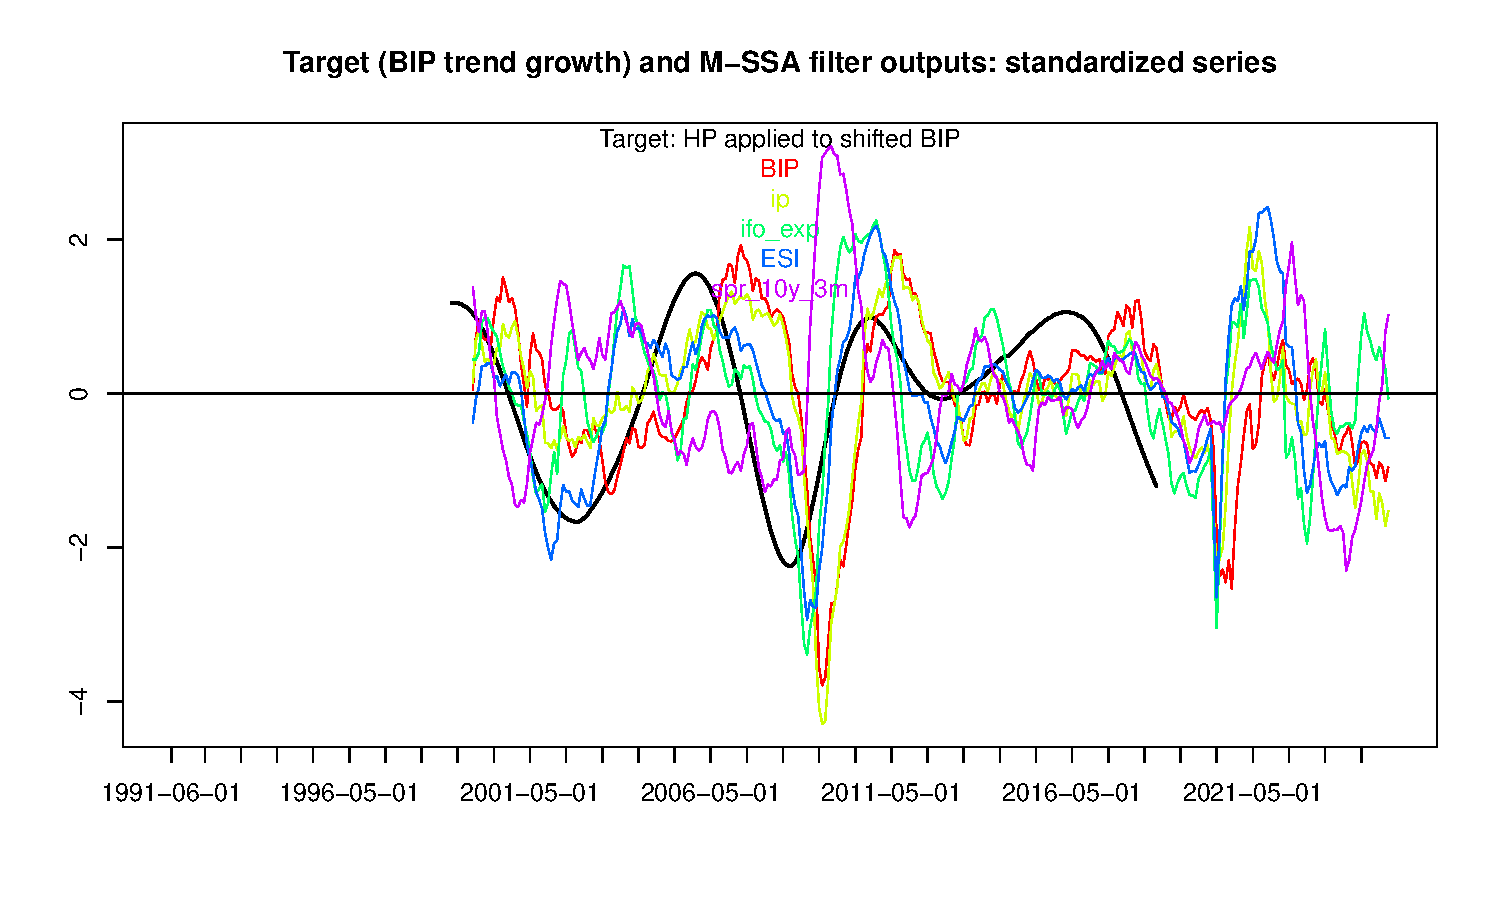
\includegraphics[height=3in, width=4in]{M_SSA_output_1.pdf}\caption{MA-inversion of VARMA\label{cor}}\end{center}\end{figure}\end{frame}


\begin{frame} {BIP-Trend (black) and M-SSA: BIP and ip Outputs}
\begin{figure}[H]\begin{center}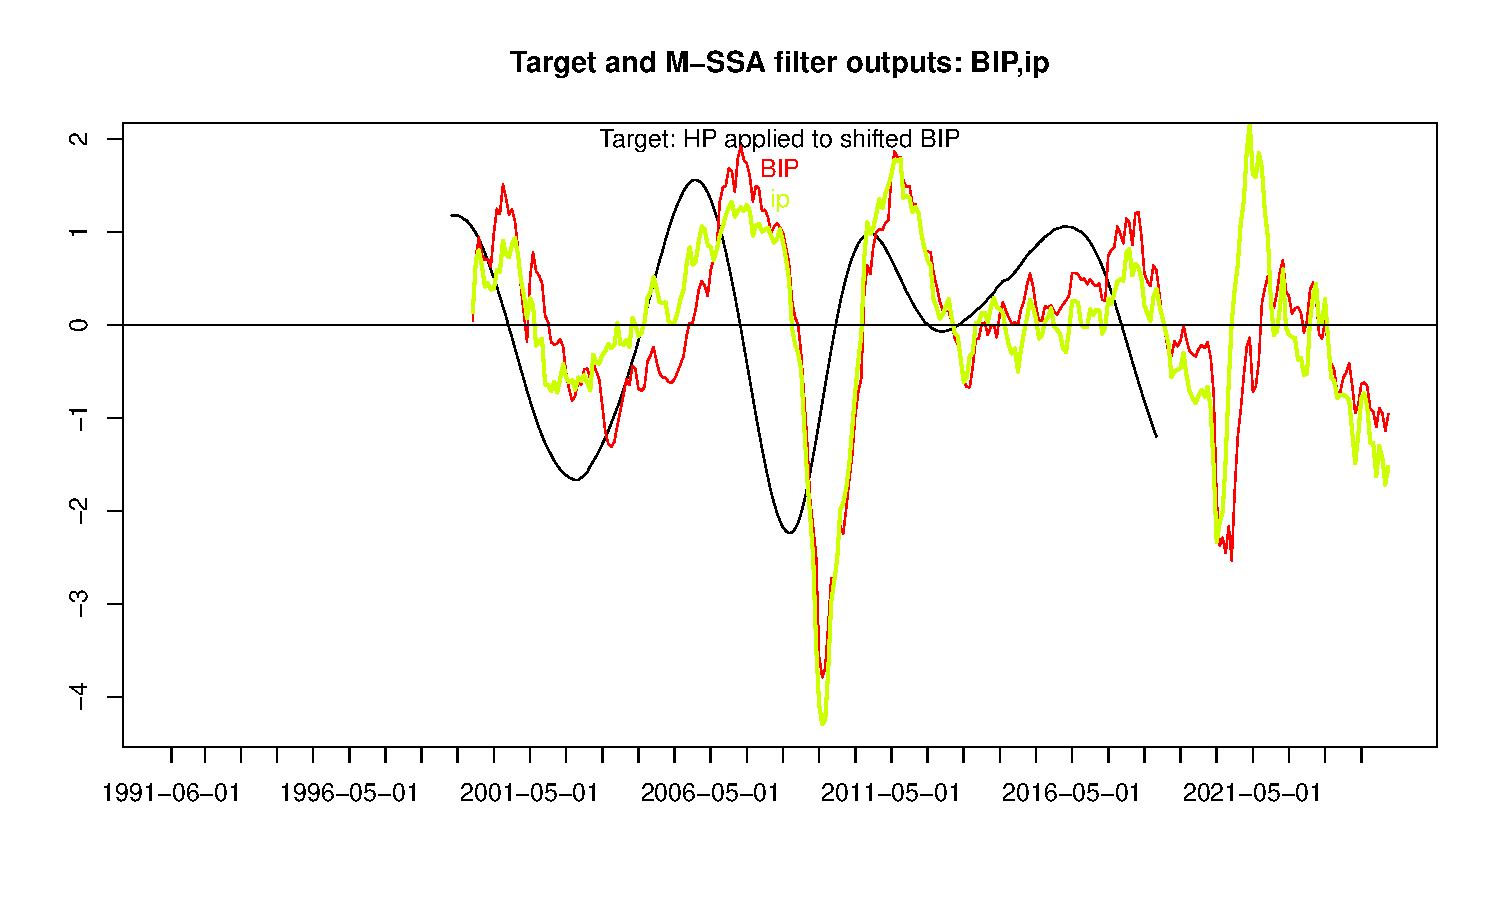
\includegraphics[height=3in, width=4in]{M_SSA_output_15.pdf}\caption{MA-inversion of VARMA\label{cor}}\end{center}\end{figure}\end{frame}


\begin{frame} {BIP-Trend (black) and M-SSA: BIP and ESI Outputs}
\begin{figure}[H]\begin{center}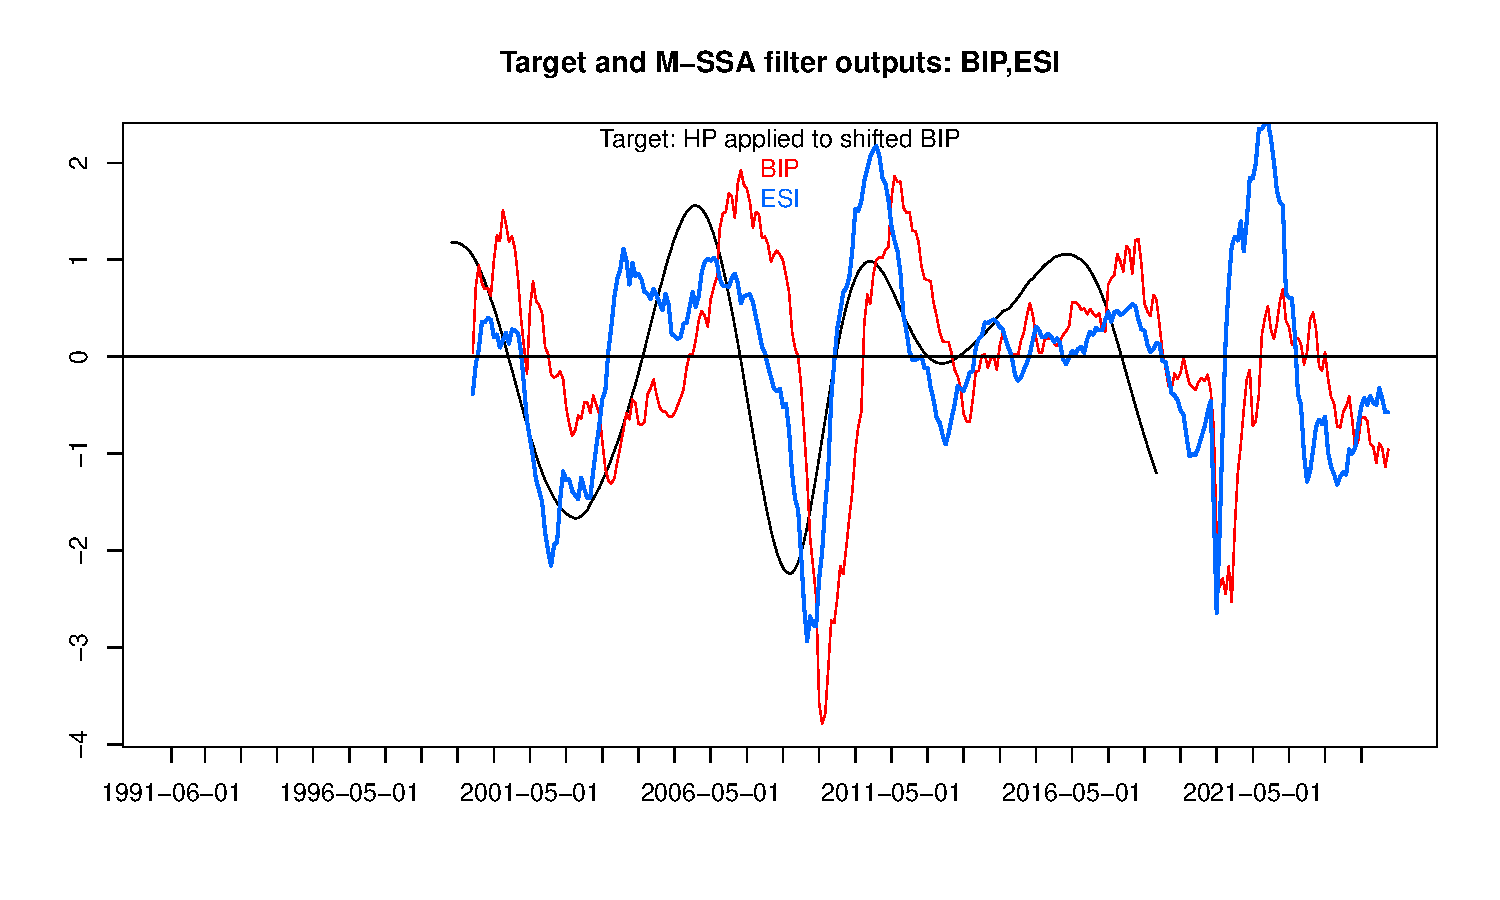
\includegraphics[height=3in, width=4in]{M_SSA_output_2.pdf}\caption{MA-inversion of VARMA\label{cor}}\end{center}\end{figure}\end{frame}


\begin{frame} {BIP-Trend (black) and M-SSA: BIP and ifo-exp Outputs}
\begin{figure}[H]\begin{center}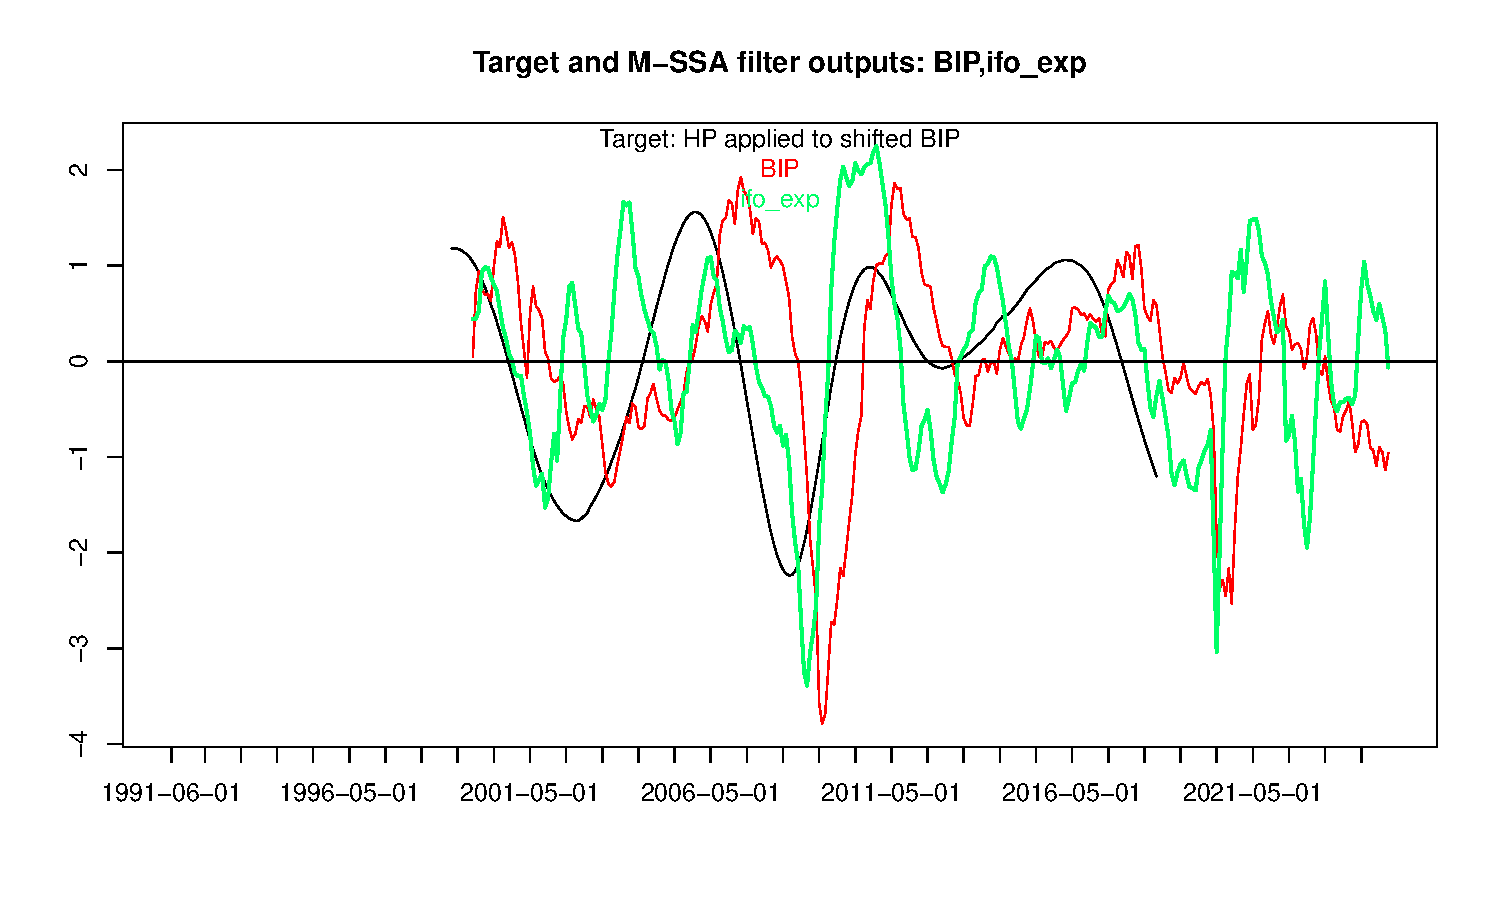
\includegraphics[height=3in, width=4in]{M_SSA_output_3.pdf}\caption{MA-inversion of VARMA\label{cor}}\end{center}\end{figure}\end{frame}


\begin{frame} {BIP-Trend (black) and M-SSA: BIP and spread Outputs}\label{spr_mssa_o}
\begin{figure}[H]\begin{center}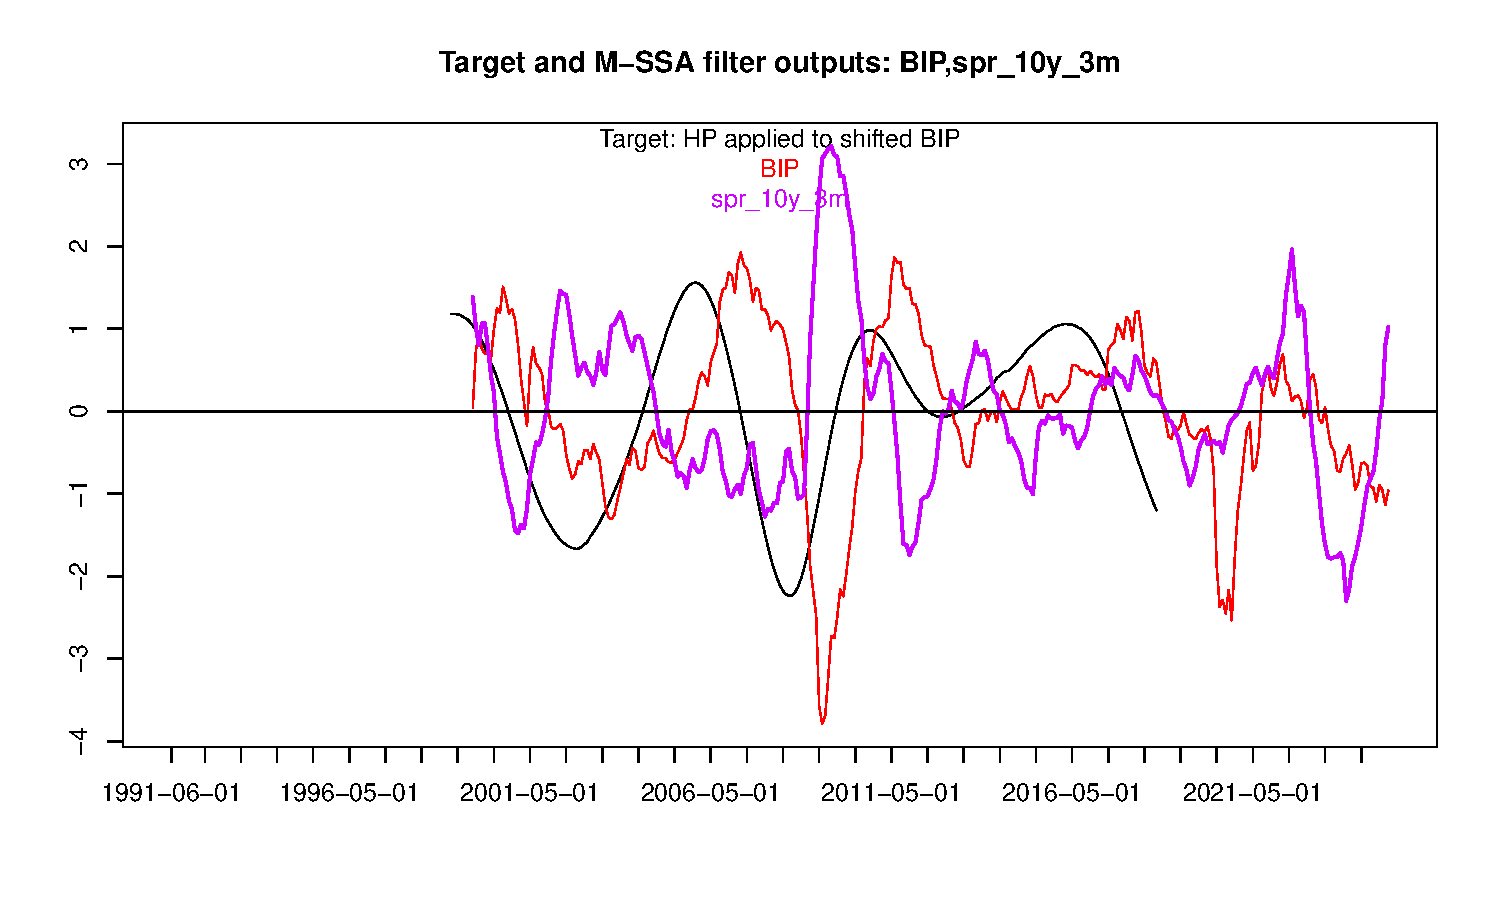
\includegraphics[height=3in, width=4in]{M_SSA_output_4.pdf}\caption{MA-inversion of VARMA\label{cor}}\end{center}\end{figure}\end{frame}


\begin{frame} {Findings}
\begin{itemize}
\item M-SSA BIP (red) is lagging target (black) due to its (largest) publication lag
\item M-SSA ip (yellow-green) is also lagging but less than M-SSA BIP
\item M-SSA ESI (blue) is both `fast' (left-shifted) and smooth: this explains the large target correlation reported in the above table(s)
\item M-SSA ifo-exp (green) is fastest but overlaid with `noisy' cycles
\item Spread (violet) does not seem to correlate with target (black) 
\end{itemize}
\end{frame}






\section{Addressing Retardation (and Smoothness)}


\frame{\sectionpage}

\subsection{Forecast Excess}

\begin{frame} {Addressing Retardation and Smoothness (HT)}
\begin{itemize}
\item Stronger smoothing generally signifies a more pronounced retardation (right shift; lag): dilemma
\item \emph{Retardation} of our filter designs can be addressed by \emph{increasing the forecast horizon} $h$ to $h+\delta$, where $\delta\geq 0$
\begin{itemize}
\item We here illustrate filters with \emph{forecast excesses} $\delta=0,3,6,12,18$ and 24 ($h=3$ is maintained)
\end{itemize}
\item In general, \textbf{increasing} $\delta$ leads ceteris paribus to a \textbf{left-shift} of the predictors (smaller retardation) and to \textbf{noisier} filters with \textbf{smaller HT} (more zero-crossings). 
\item However, in the \textbf{M-SSA} framework we can control and \textbf{fix the HT}: the M-SSA predictor will maintain a fixed HT irrespective of $\delta$
\item Therefore, we can \textbf{maintain smoothness} while \textbf{mitigating retardation} to some extent (by extending the classic forecast dilemma to a more general forecast trilemma, see SSA paper) 
\end{itemize}

\end{frame}


\subsection{M-SSA-BIP and Variable Forecast Excess}


\begin{frame} {Addressing Retardation and Smoothness (HT)}
\begin{itemize}
\item In the previous slides we saw that M-SSA-BIP (the output of M-SSA corresponding to the shifted BIP-target: red lines) was lagging
\item The next two plots illustrate the effect of $\delta=0,3,6,12,18,24$ on M-SSA-BIP  for the whole sample (first plot) and for the financial crisis and the pandemic (second plot)
\begin{itemize}
\item We \textbf{fix} the target, i.e. M-SSA-BIP, and we \textbf{vary} $\delta$
\item Later, we will compare \textbf{all} M-SSA outputs (not only M-SSA-BIP) for  $\delta=12$ \textbf{fixed}
\item Finally, we will analyze \textbf{all combinations}: all selected M-SSA outputs for all selected $\delta$
\item Note: we do not display the M-MSE outputs which are noisier (more `false alarms'), see the ip-case for reference
\end{itemize}
\item For ease of visual inspection we apply \textbf{standardization} (equivalent to filter calibration)
\end{itemize}
\end{frame}


















\begin{frame} {Look Ahead: Effect of $\delta$ on Advancement (Left Shift) of M-SSA-BIP }
\begin{figure}[H]\begin{center}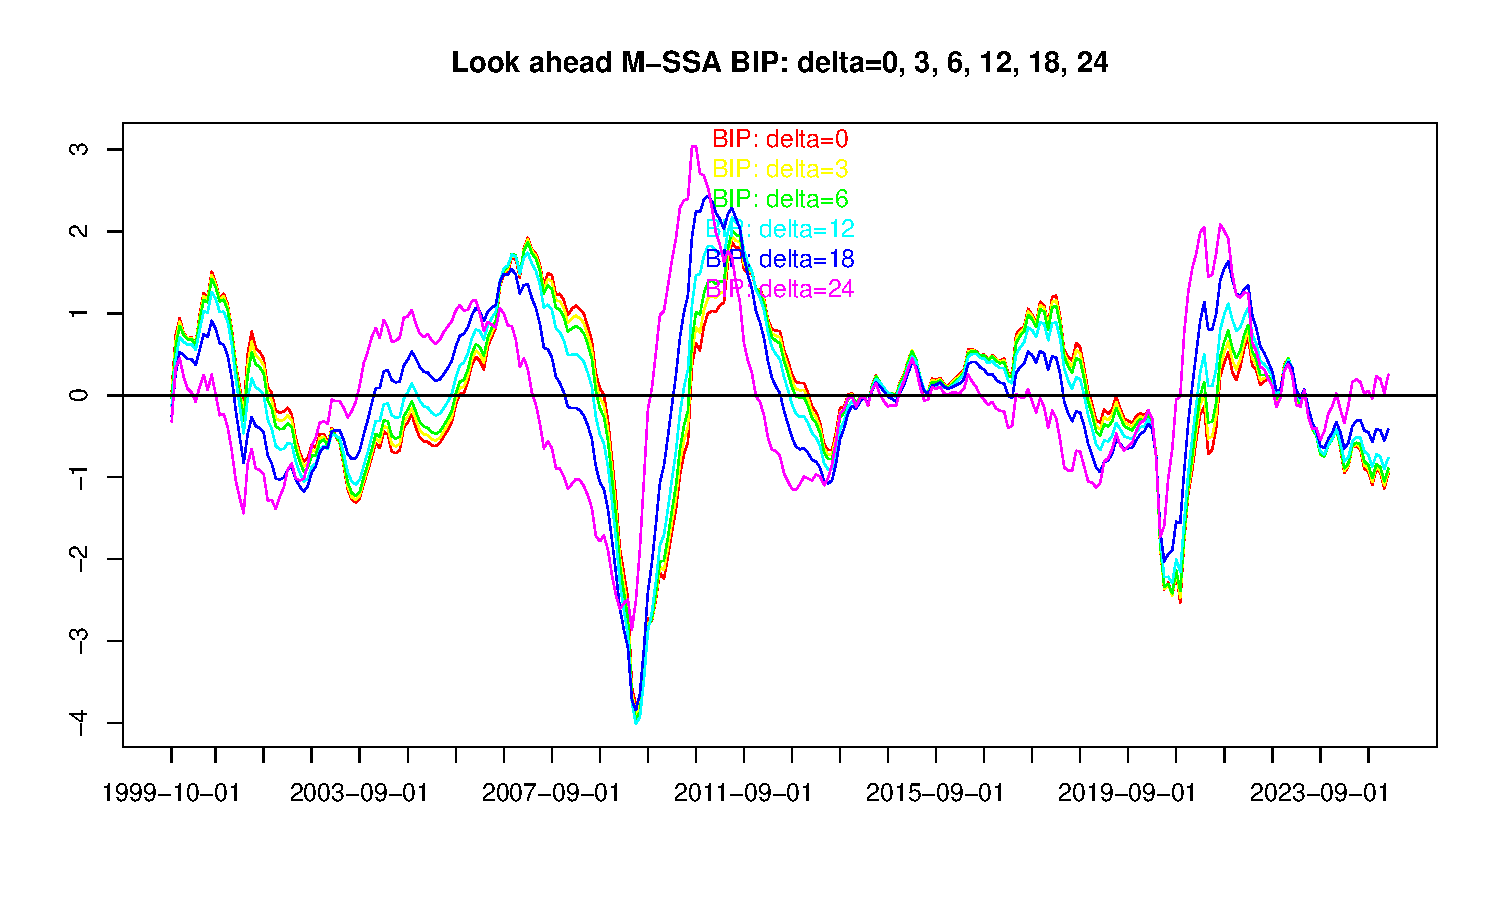
\includegraphics[height=3in, width=4in]{look_ahead_ssa_1.pdf}\caption{Effect of look ahead delta on  left-shift/advancement of M-SSA\label{cor}}\end{center}\end{figure}\end{frame}

\begin{frame} {Financial Crisis (left) and Pandemic (right)}
\begin{figure}[H]\begin{center}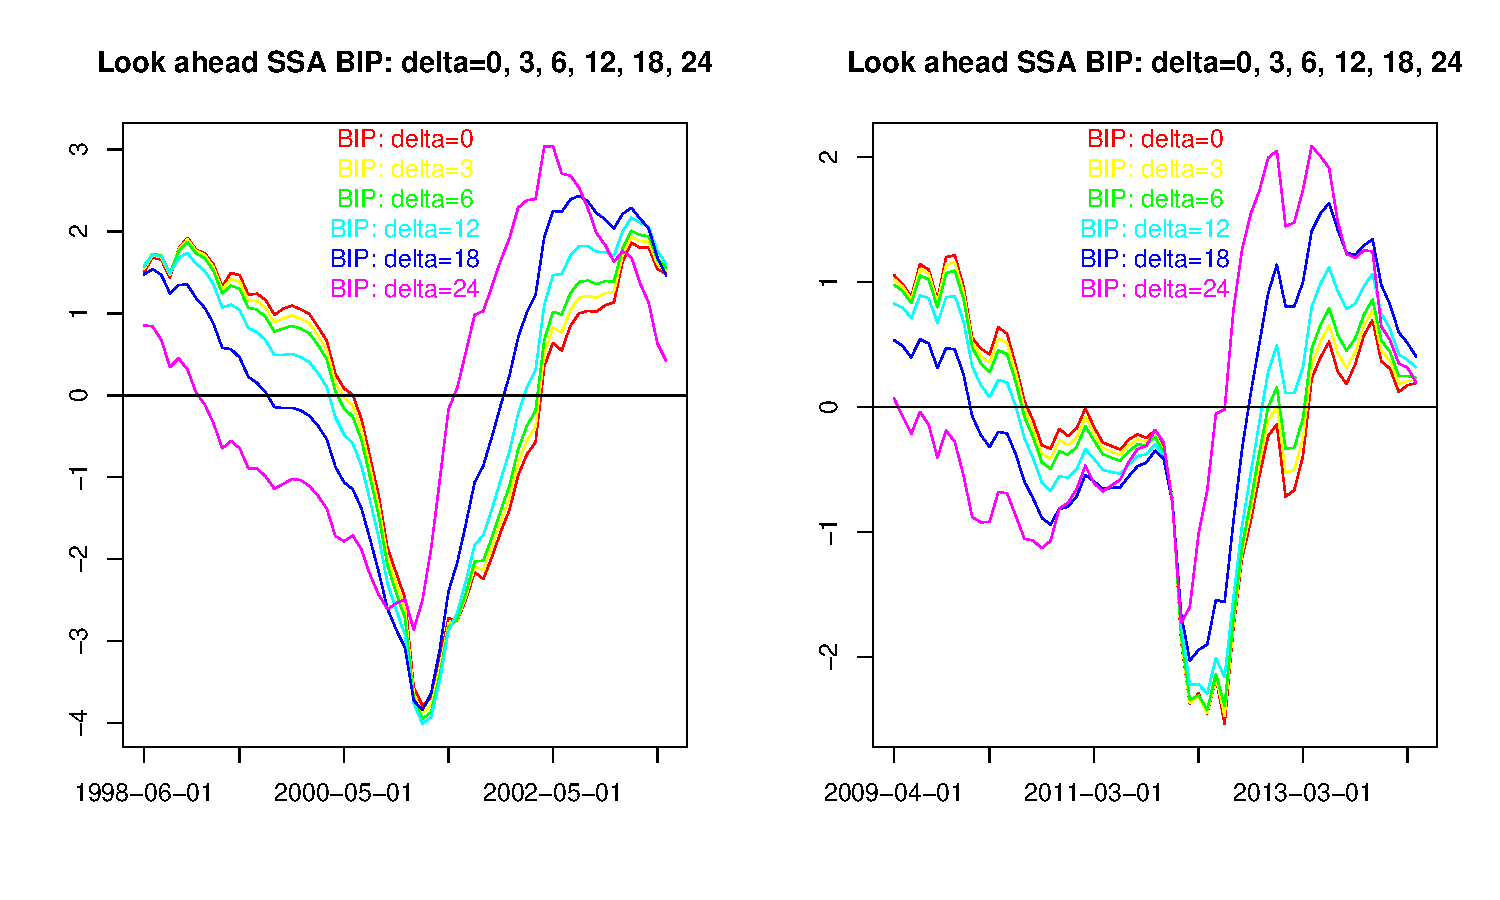
\includegraphics[height=3in, width=4in]{look_ahead_ssa_2.pdf}\caption{Effect of look ahead delta on  left-shift/advancement of M-SSA\label{cor}}\end{center}\end{figure}\end{frame}







\begin{frame} {Findings}
\begin{itemize}
\item The main effect of $\delta=3, 6, 12, 18, 24$ on \textbf{M-SSA-BIP} is a \textbf{left-shift} of the filter output 
\begin{itemize}
\item A larger $\delta$  means that zero-crossings at onset and end of crises are detected earlier(advancement, left-shift)
\item Note that M-SSA keeps the (expected) HT fixed for increasing $\delta$ (in contrast to M-MSE which becomes noisier, see slides of ip-case)
\item The filters are also subject to zero-shrinkage for increasing $\delta$ (but this effect is masked by the standardization) 
\end{itemize}
\item We report \textbf{sample HTs} for M-MSE and M-SSA filters as a function of $\delta$: see the table on the next slide

\end{itemize}

\end{frame}





\begin{frame} {Holding-Times}\label{htzc2}



% latex table generated in R 4.2.2 by xtable 1.8-4 package
% Sat Feb 15 08:41:28 2025
\begin{table}[ht]
\centering
\begin{tabular}{rrrrrr}
  \hline
 & delta=0 & delta=3 & delta=6 & delta=12 & delta=18 \\ 
  \hline
M-MSE & 9.20 & 9.80 & 8.70 & 7.60 & 6.90 \\ 
  M-SSA & 16.00 & 13.20 & 13.80 & 16.90 & 19.00 \\ 
   \hline
\end{tabular}
\caption{Holding times of M-MSE and M-SSA for various values of look ahead parameter $\delta$} 
\label{perf_var1}
\end{table}\begin{itemize}
\item The above HTs of M-SSA should be compared with the univariate SSA on slide \eqref{htzc1}, first row, last column: by construction expected numbers should match (sample HTs are subject to random deviations)

\end{itemize}

\end{frame}



\begin{frame} {Findings}
\begin{itemize}
\item M-SSA is substantially smoother (less crossings, i.e., less false alarms)
\item The \emph{expected} HT is independent of $\delta$ 
\begin{itemize}
\item The differences in the above \emph{sample} HTs (of M-SSA) reveal mainly \emph{finite sample} variations
\item The \emph{sample} HTs converge to the  \emph{fixed expected} value in sufficiently long samples (see SSA tutorial)
\end{itemize}

%\item We now compare graphically M-MSE and M-SSA for $\delta=12$: zero-crossings are marked by corresponding colored vertical lines

\end{itemize}

\end{frame}




%\begin{frame} {Holding-Times: $\delta=24$}
%<<label=z_box_plot_pure_mba_2.pdf,echo=FALSE,results=tex>>=
%file = "ht_look_ahead.pdf"
%cat("\\begin{figure}[H]")
%cat("\\begin{center}")
%cat("\\includegraphics[height=3in, width=4in]{", file, "}\n",sep = "")
%cat("\\caption{Effect of look ahead delta on  left-shift/advancement of MSE", sep = "")
%cat("\\label{cor}}", sep = "")
%cat("\\end{center}")
%cat("\\end{figure}")
%@
%\end{frame}





\begin{frame} {Effect of $\delta$ on Target Correlation and Sign Accuracy}\label{sample_target_cor3}
\begin{itemize}
\item We analyze the effect of $\delta$ on the target correlation and the sign accuracy, see the following table. 
\end{itemize}

% latex table generated in R 4.2.2 by xtable 1.8-4 package
% Sat Feb 15 08:41:28 2025
\begin{table}[ht]
\centering
\begin{tabular}{rrr}
  \hline
 & Target correlation & Sign accuracy \\ 
  \hline
delta=0 & 0.17 & 0.62 \\ 
  delta=3 & 0.22 & 0.63 \\ 
  delta=6 & 0.27 & 0.64 \\ 
  delta=12 & 0.38 & 0.68 \\ 
  delta=18 & 0.56 & 0.77 \\ 
  delta=24 & 0.69 & 0.77 \\ 
   \hline
\end{tabular}
\caption{Target correlations (first column) and sign accuracy (second column) of M-SSA-BIP for various $\delta\geq 0$ values } 
\label{perf_var1}
\end{table}\begin{itemize}
\item Note: the target correlation for $\delta=0$ (first row, first column) corresponds to slide \eqref{sample_target_cor2} (first row, second column)
\end{itemize}


\end{frame}








\begin{frame} {Effect of $\delta$ on Filter Weights}
\begin{figure}[H]\begin{center}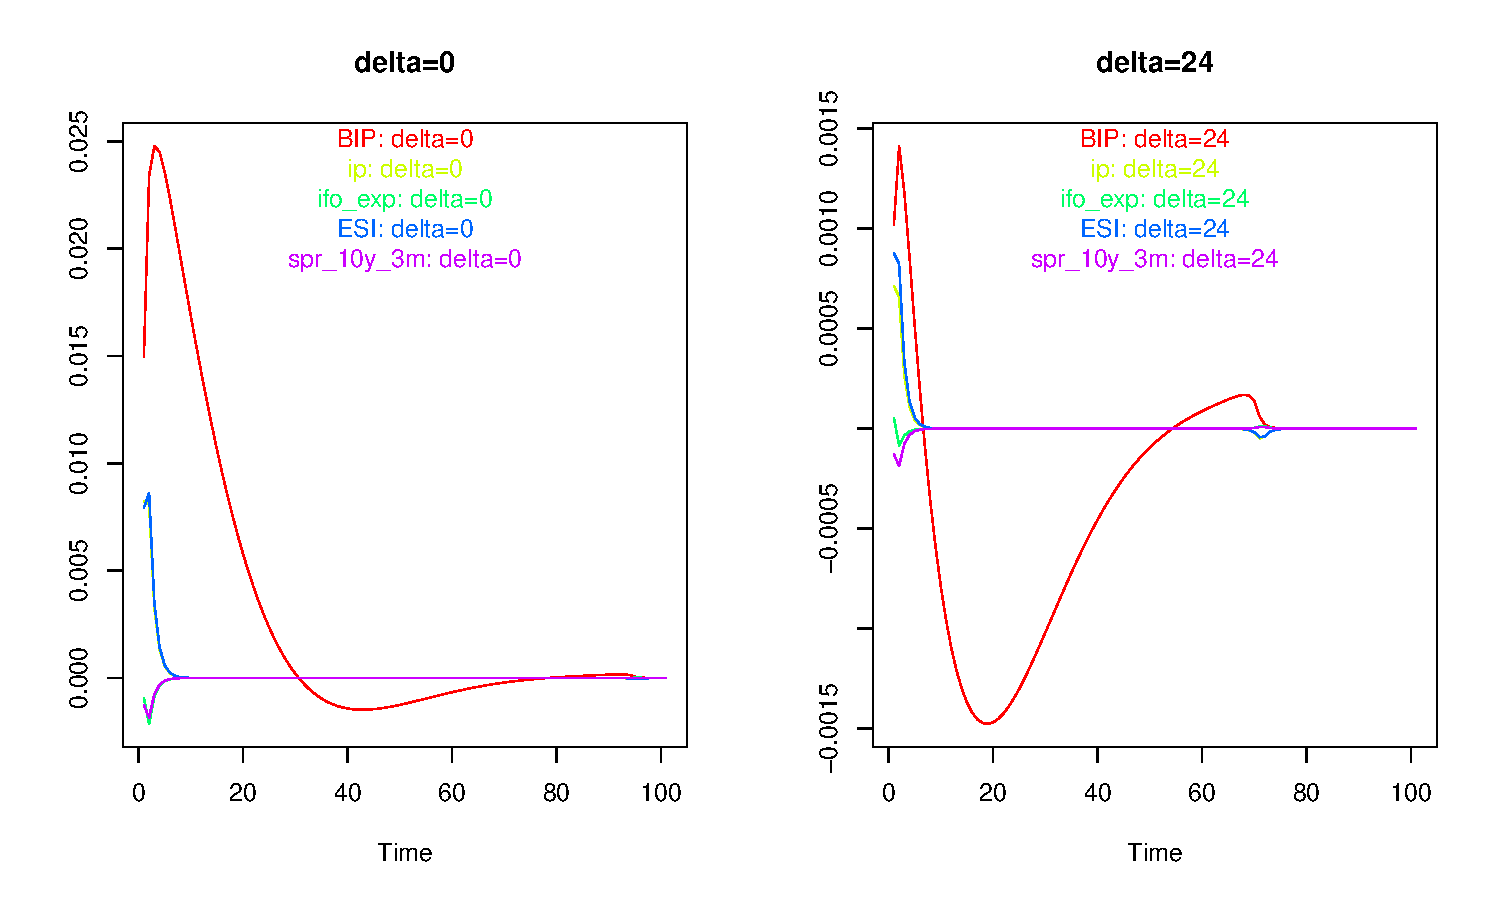
\includegraphics[height=3in, width=4in]{look_ahead_ssa_6.pdf}\caption{Effect of look ahead delta on  left-shift/advancement of M-SSA\label{cor}}\end{center}\end{figure}\end{frame}


\begin{frame} {Same as Previous Slide but MA-Inversion of Filter}
\begin{figure}[H]\begin{center}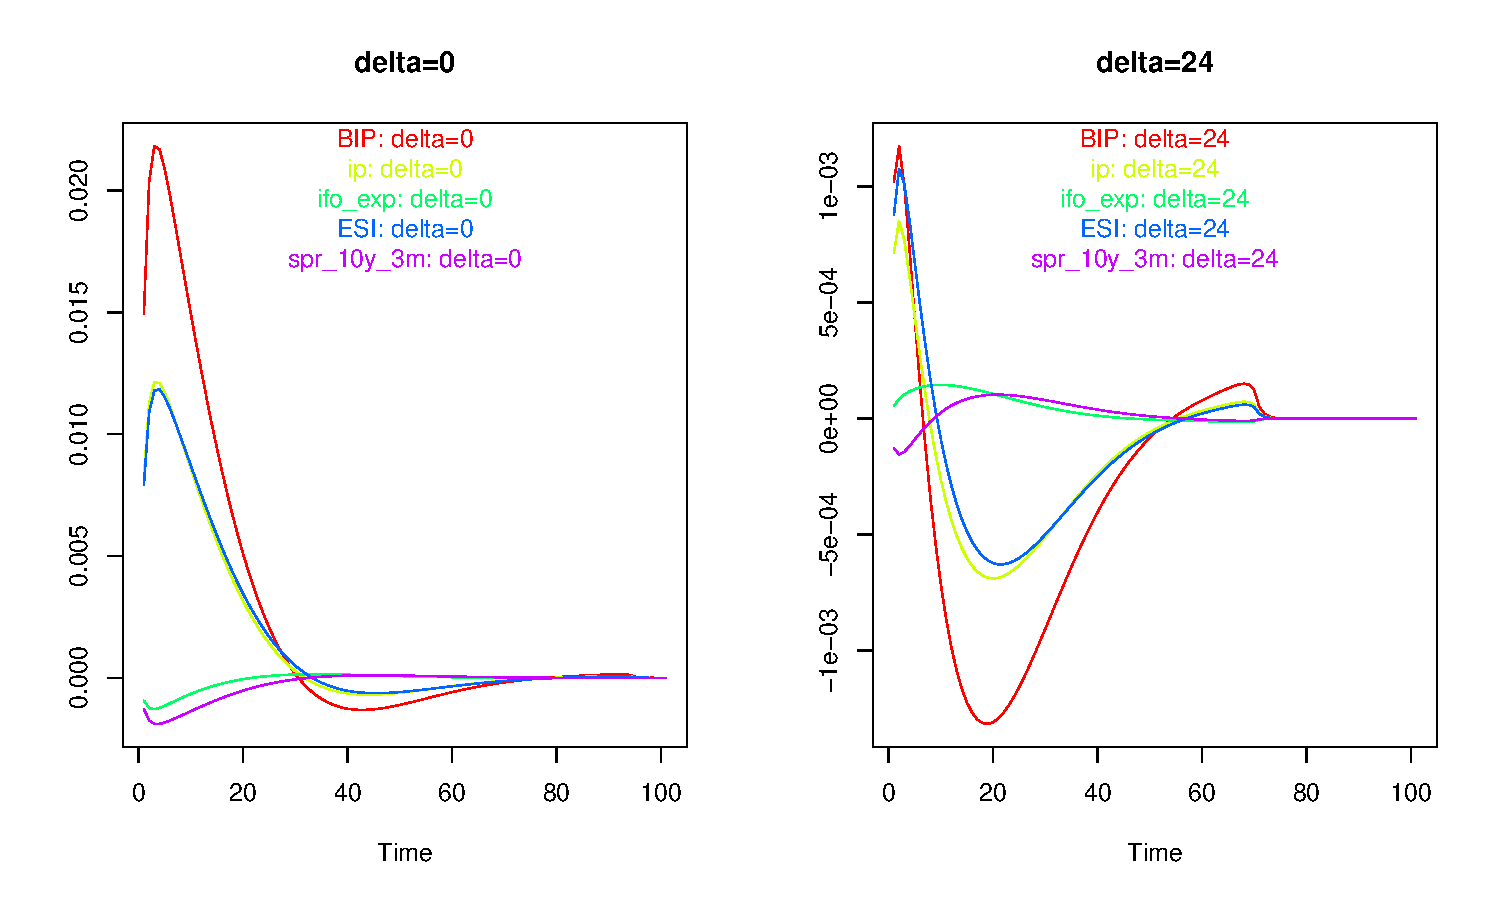
\includegraphics[height=3in, width=4in]{look_ahead_ssa_7.pdf}\caption{Effect of look ahead delta on  left-shift/advancement of M-SSA\label{cor}}\end{center}\end{figure}\end{frame}





\begin{frame} {Findings}
\begin{itemize}
\item The original M-SSA-BIP, based on $\delta=0$, was lagging (due in part to VARMA model misspecification)
\item Increasing $\delta$ leads to substantial improvements of \emph{target correlation} and \emph{sign accuracy}
\item Increasing $\delta$ signifies a \textbf{left-shift} of the filter outputs: this left-shift \emph{explains} mainly the improvement  
\item Increasing $\delta$ induces a zero-shrinkage of the filter weights and a modification of the general decay-pattern, see the plots just above
\begin{itemize}
\item The shrinkage of the filter coefficients does not affect \emph{standardized} filter outputs
\item The different decay pattern affects the left-shift of the (standardized) filter outputs; but it does not affect the (expected) HT
\end{itemize}
\end{itemize}
\end{frame}





\subsection{All M-SSA Outputs and Fixed $\delta=12$}

\begin{frame} {Variable (All) M-SSA Targets and Fixed Forecast Excess}
\begin{itemize}
\item In the above slides we showed the effect of $\delta$ on the M-SSA-BIP output 
\item We now consider \textbf{all} M-SSA outputs for \textbf{fixed} $\delta=12$ (all M-SSA outputs for $\delta=0$ were analyzed previously)
\end{itemize}

\end{frame}


\begin{frame} {All M-SSA Outputs for Fixed $\delta=12$}
\begin{itemize}
\item In contrast to the previous slides, we now \textbf{fix} $\delta:=12$ and we analyze \textbf{all} M-SSA outputs for that $\delta$
\item On the next slide we now display and compare the corresponding look-ahead M-SSA outputs for $\delta=12$  
\item For reference, we also include BIP-trend, i.e., the acausal HP applied to BIP-shifted (black line)
\item For easier visual inspection all series are standardized (equivalent to filter calibration)
\end{itemize}

\end{frame}


\begin{frame} {All M-SSA Outputs for (Fixed) $\delta=12$}
\begin{figure}[H]\begin{center}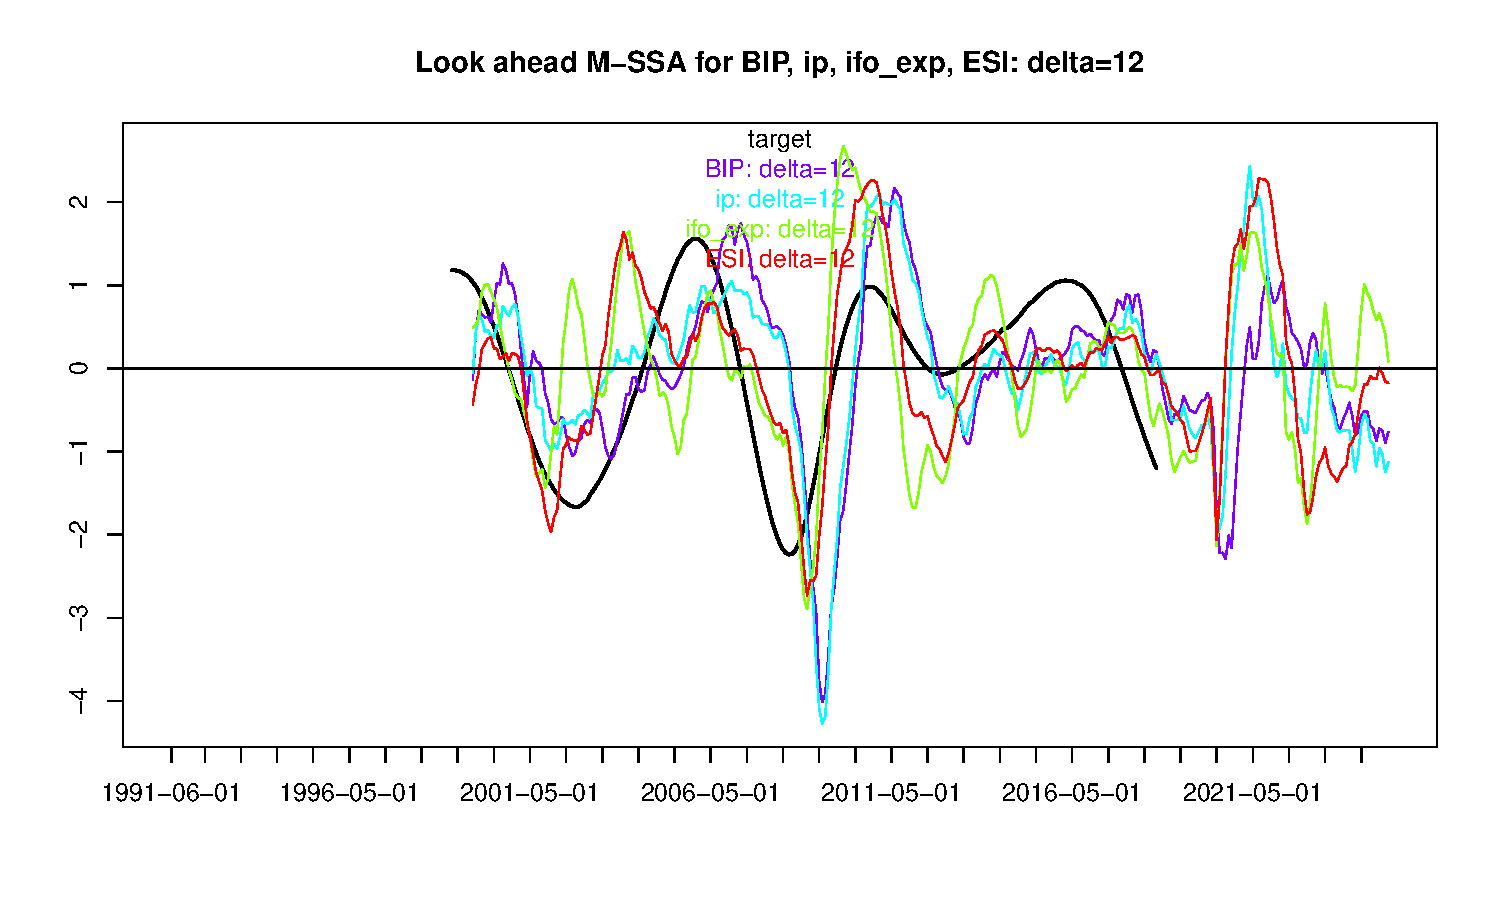
\includegraphics[height=3in, width=4in]{look_ahead_ssa_3.pdf}\caption{Effect of look ahead delta on  left-shift/advancement of M-SSA\label{cor}}\end{center}\end{figure}\end{frame}

\begin{frame} {Findings}
\begin{itemize}
\item M-SSA outputs for ESI (red), ifo-exp (green), ip (cyan) and BIP (violet) differ mainly during the financial crisis, where especially the former two are left-shifted and faster 
\begin{itemize}
\item The financial crisis cannot be reconciled with the VARMA-model (misspecification) which explains the lesser performance of the BIP M-SSA output in all previous comparisons (details omitted).
\end{itemize}
\item Towards the sample end, M-SSA ifo-exp (and to some extent M-SSA ESI) suggest evidence of a  \textbf{recovery} whereas M-SSA ip and BIP still indicate negative growth.

\end{itemize}

\end{frame}







\begin{frame} {Sign Accuracies}\label{signaac1}
\begin{itemize}
\item In order to complete our evaluation metrics, the table below reports \textbf{sign accuracies} of the M-SSA outputs, i.e., the (sample) probability that a predictor matches the sign of the target (BIP-trend, black line in previous plot)
\end{itemize}


% latex table generated in R 4.2.2 by xtable 1.8-4 package
% Sat Feb 15 08:41:28 2025
\begin{table}[ht]
\centering
\begin{tabular}{rlllll}
  \hline
 & BIP & ip & ifo\_exp & ESI & spr\_10y\_3m \\ 
  \hline
sign acc. & 0.68(0.03) & 0.68(0.03) & 0.65(0.03) & 0.74(0.03) & 0.39(0.03) \\ 
   \hline
\end{tabular}
\caption{Sign accuracies of M-SSA outputs for fixed $\delta=12$ with standard errors in parentheses} 
\label{perf_var1}
\end{table}\begin{itemize}
\item For fixed $\delta=12$,  ESI (red line in previous plot) is best, followed closely by ip, BIP and ifo-exp. The sign accuracy of spread is below $50\%$ 
\end{itemize}

\end{frame}


\subsection{All Combinations  of M-SSA Outputs and of Forecast Excess(es)}



\begin{frame} {All Combinations of Forecast Excess and M-SSA Outputs}
\begin{itemize}
\item Up yet we considered specific combinations of forecast excess and M-SSA outputs
\item The tables in the following three slides report sample \emph{sign-accuracy}, sample \emph{target correlation}  and sample \emph{holding-times} for \textbf{all combinations} of M-SSA outputs and $\delta$
\begin{itemize}
\item Sign-accuracy and sample correlation are evaluated against BIP-trend, i.e., acausal HP applied to BIP-shift
\end{itemize}
\end{itemize}
\end{frame}



\begin{frame} {Sample Sign Accuracy}\label{signaac2}
% latex table generated in R 4.2.2 by xtable 1.8-4 package
% Sat Feb 15 08:41:28 2025
\begin{table}[ht]
\centering
\begin{tabular}{rrrrrr}
  \hline
 & BIP & ip & ifo\_exp & ESI & spr\_10y\_3m \\ 
  \hline
delta=0 & 0.62 & 0.64 & 0.68 & 0.74 & 0.43 \\ 
  delta=3 & 0.63 & 0.65 & 0.67 & 0.73 & 0.42 \\ 
  delta=6 & 0.64 & 0.68 & 0.67 & 0.74 & 0.42 \\ 
  delta=12 & 0.68 & 0.68 & 0.65 & 0.74 & 0.39 \\ 
  delta=18 & 0.77 & 0.74 & 0.61 & 0.67 & 0.36 \\ 
  delta=24 & 0.77 & 0.71 & 0.50 & 0.52 & 0.42 \\ 
   \hline
\end{tabular}
\caption{Sign accuracies of all combinations of M-SSA outputs (columns) and forecast excesses $\delta$ (rows): the sign accuracy is referenced against BIP-trend} 
\label{perf_var1}
\end{table}\end{frame}



\begin{frame} {Sample Target Correlation}\label{sample_target_cor4}
% latex table generated in R 4.2.2 by xtable 1.8-4 package
% Sat Feb 15 08:41:28 2025
\begin{table}[ht]
\centering
\begin{tabular}{rrrrrr}
  \hline
 & BIP & ip & ifo\_exp & ESI & spr\_10y\_3m \\ 
  \hline
delta=0 & 0.17 & 0.28 & 0.47 & 0.66 & -0.09 \\ 
  delta=3 & 0.22 & 0.31 & 0.45 & 0.65 & -0.10 \\ 
  delta=6 & 0.27 & 0.34 & 0.43 & 0.63 & -0.12 \\ 
  delta=12 & 0.38 & 0.41 & 0.38 & 0.58 & -0.18 \\ 
  delta=18 & 0.56 & 0.52 & 0.23 & 0.41 & -0.31 \\ 
  delta=24 & 0.69 & 0.54 & -0.10 & -0.02 & -0.40 \\ 
   \hline
\end{tabular}
\caption{Target correlations of all combinations of M-SSA outputs (columns) and forecast excesses $\delta$ (rows): the target correlation is referenced against BIP-trend} 
\label{perf_var1}
\end{table}\end{frame}


\begin{frame} {Sample HT}\label{htzc3}
% latex table generated in R 4.2.2 by xtable 1.8-4 package
% Sat Feb 15 08:41:29 2025
\begin{table}[ht]
\centering
\begin{tabular}{rrrrrr}
  \hline
 & BIP & ip & ifo\_exp & ESI & spr\_10y\_3m \\ 
  \hline
delta=0 & 16.00 & 11.26 & 11.69 & 19.00 & 25.33 \\ 
  delta=3 & 13.22 & 11.26 & 12.67 & 21.71 & 25.33 \\ 
  delta=6 & 13.82 & 10.48 & 12.67 & 19.00 & 19.00 \\ 
  delta=12 & 16.89 & 12.67 & 11.69 & 19.00 & 21.71 \\ 
  delta=18 & 19.00 & 15.20 & 11.69 & 14.48 & 13.82 \\ 
   \hline
\end{tabular}
\caption{Sample holding times of all combinations of M-SSA outputs (columns) and forecast excesses $\delta$ (rows)} 
\label{perf_var1}
\end{table}\begin{itemize}
\item Remarks:
\begin{itemize}
\item Expected HTs change along columns (from left to right) but are fixed along rows (top to bottom)
\item Sample HTs in the table follow this pattern (though subject to random variation)
\end{itemize}
\end{itemize}

\end{frame}



\begin{frame} {Findings}
\begin{itemize}
\item M-SSA outputs of lagging series (such as BIP and ip: first two columns in above tables) perform better for larger $\delta$
\item M-SSA outputs of coincident series (ESI, ifo-exp, columns 3 and 4) perform best for small values of $\delta$
\begin{itemize}
\item M-SSA ifo-exp is systematically outperformed by M-SSA ESI
\end{itemize}
\item The above findings are intuitively appealing/interpretable
\item M-SSA output of spread is not a good predictor of the target
\item \textbf{Summary}: we can combine M-SSA \textbf{BIP} and \textbf{ip} with \textbf{large} $\delta$ and M-SSA \textbf{ESI} for \textbf{small} $\delta$
\end{itemize}
\end{frame}

\section{(Construction of a) Forward-Looking Consensus BIP-Predictor}

\frame{\sectionpage}


\begin{frame} {Findings}
\begin{itemize}
\item As claimed, we can combine M-SSA \textbf{BIP} and \textbf{ip} with \textbf{large} $\delta$ and M-SSA \textbf{ESI} for \textbf{small} $\delta$ to construct a forward-looking ($h=3$) BIP-predictor 
\begin{itemize}
\item The procedure cyn be extended to arbitrary $h$ (hyperparameter)
\end{itemize}
\item Given similar performances of the selected indicators we rely on an \emph{equally-weighted} `consensus' predictor
\begin{itemize}
\item Equal-weighting of \emph{standardized} predictors (standardization accounts for zero-shrinkage)
\end{itemize}
\item On the following two slides we display the selected (standardized) indicators and their cross-sectional mean,i.e., the \textbf{forward-looking consensus BIP-predictor}
\end{itemize}
\end{frame}



\begin{frame} {BIP-Trend (black) and Selected Predictors}
\begin{figure}[H]\begin{center}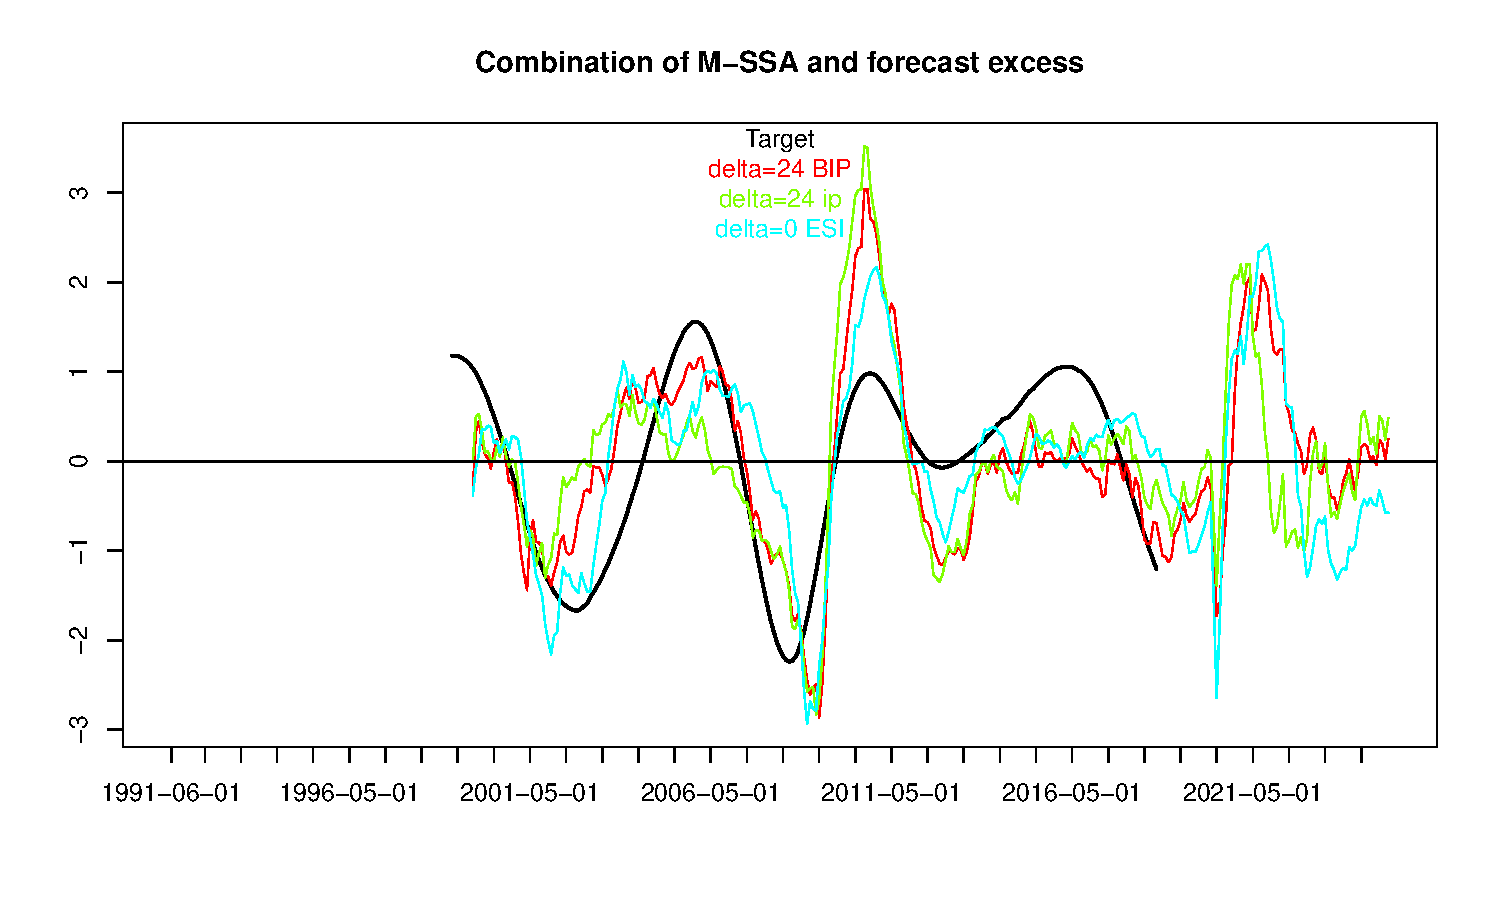
\includegraphics[height=3in, width=4in]{bip_predictor1.pdf}\caption{Effect of look ahead delta on  left-shift/advancement of M-SSA\label{cor}}\end{center}\end{figure}\end{frame}




\begin{frame} {BIP-Trend (black) and Forward-Looking Consensus BIP-Predictor}
\begin{figure}[H]\begin{center}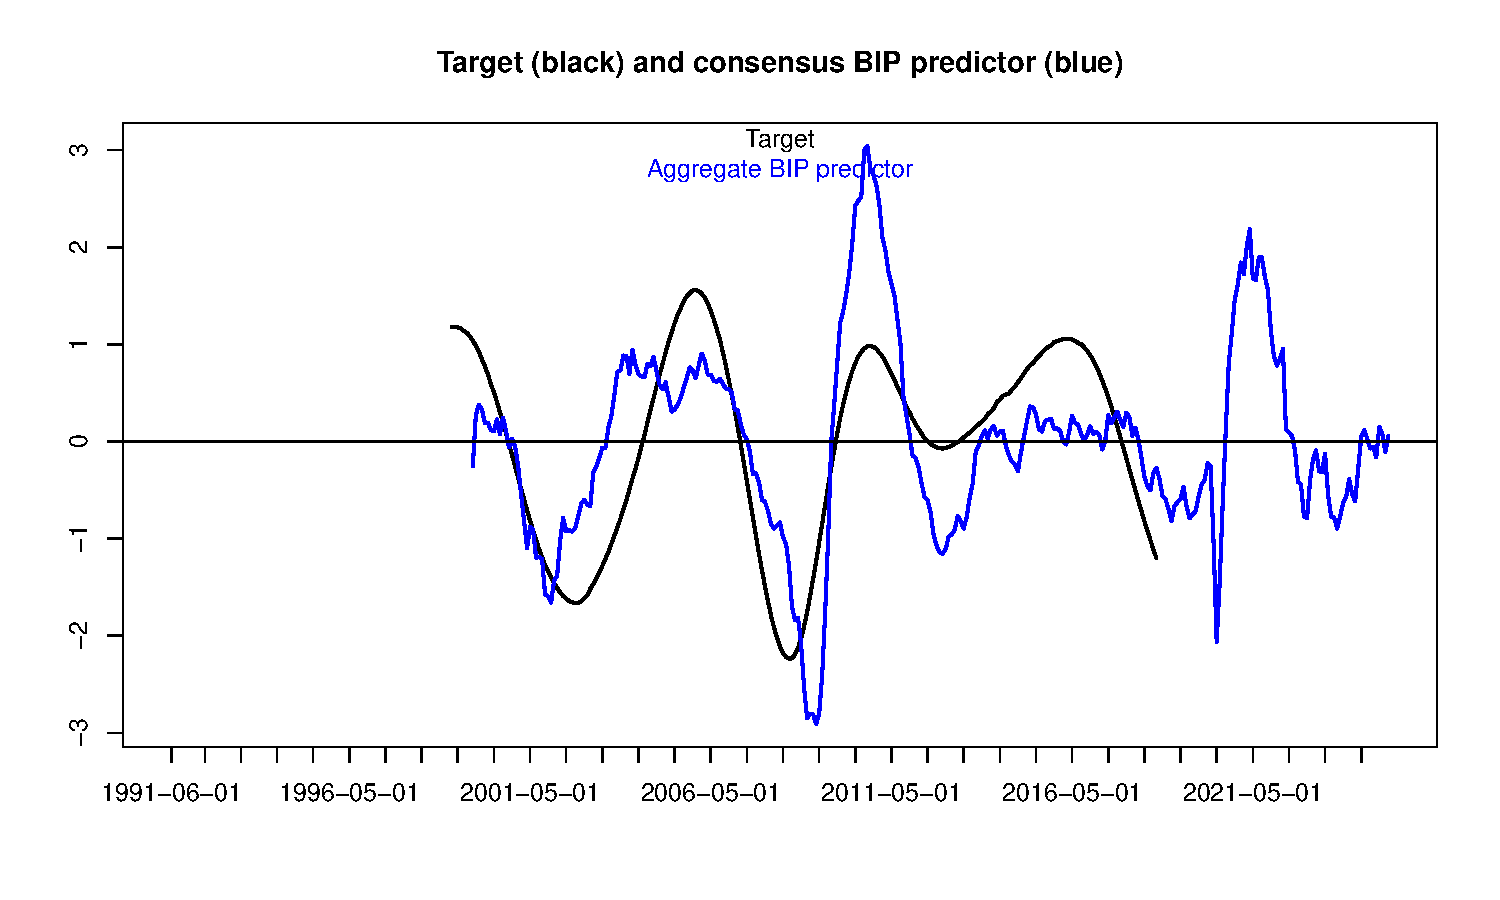
\includegraphics[height=3in, width=4in]{bip_predictor2.pdf}\caption{Effect of look ahead delta on  left-shift/advancement of M-SSA\label{cor}}\end{center}\end{figure}\end{frame}


\begin{frame} {Calibrated Forward-Looking Consensus BIP-Predictor}
\begin{itemize}
\item We can also calibrate the predictor on level and scale of BIP-returns by simple linear regression, see next slide
\item We display
\begin{itemize}
\item \textbf{Quarterly BIP} returns shifted forward by $h=3$ (black): interpolated with zero for months 2 and 3
\item \textbf{Two-sided HP} applied to shifted BIP (violet). We multiply HP by 3 to match the \emph{quarterly growth} scale of BIP
\item \textbf{Calibrated consensus} indicator with long-term mean growth (horizontal blue line) and \textbf{mean-crossings} (vertical blue lines)
\end{itemize}
\item Duration between mean-crossings is HT=13.82 ($\approx$mean of HTs of selected indicators)
\end{itemize}
\end{frame}


\begin{frame} {Calibrated Forward-Looking Consensus BIP-Predictor}
\begin{figure}[H]\begin{center}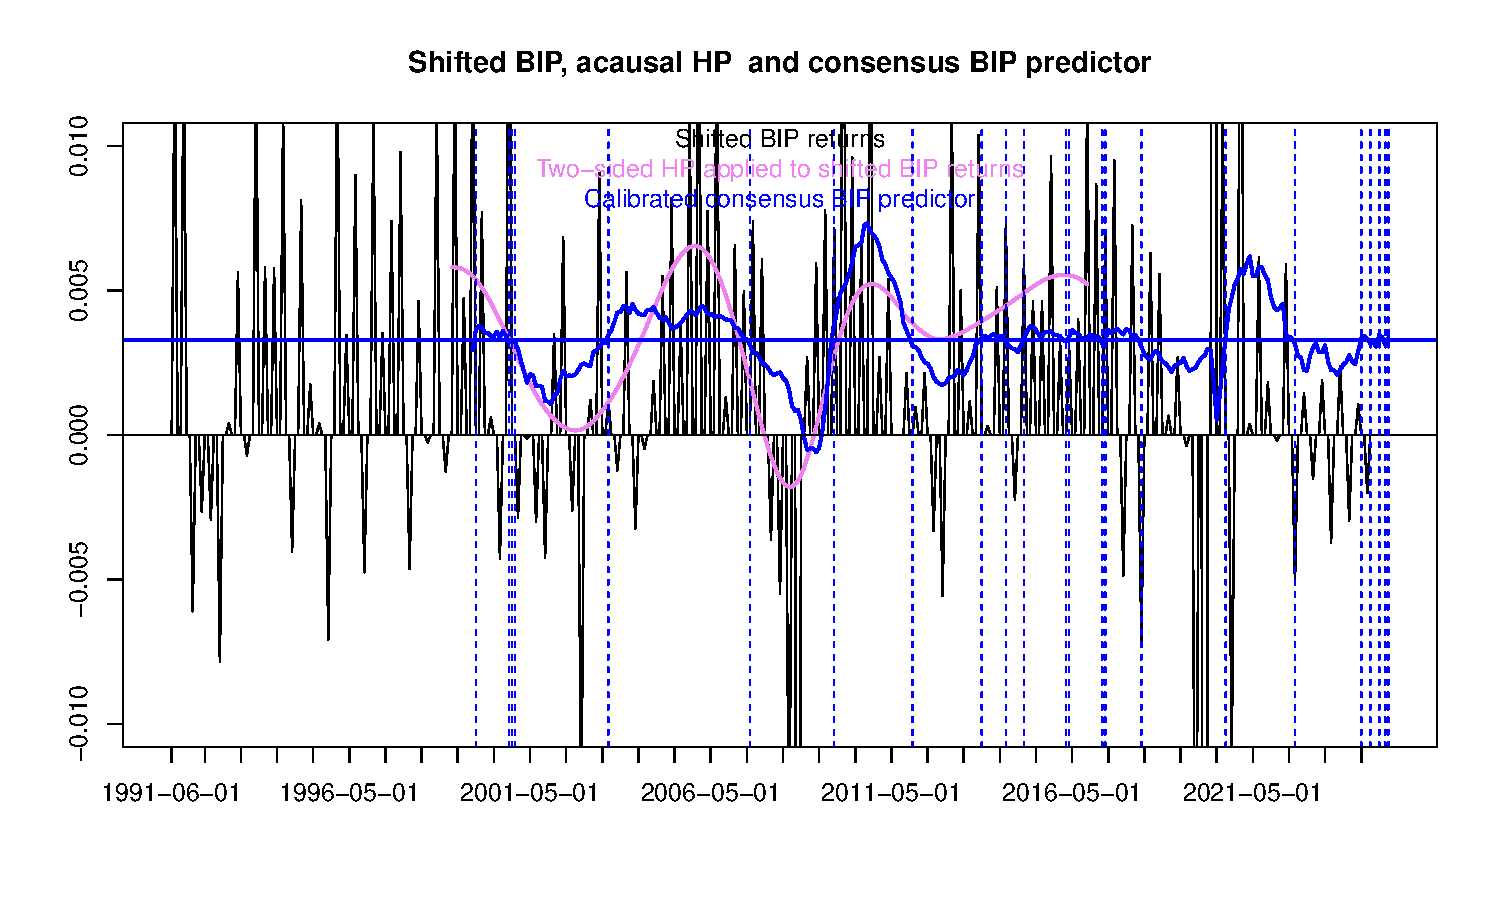
\includegraphics[height=3in, width=4in]{bip_predictor3.pdf}\caption{Effect of look ahead delta on  left-shift/advancement of M-SSA\label{cor}}\end{center}\end{figure}\end{frame}


\begin{frame} {Sensitivity to Estimation Sample }
\begin{itemize}
\item Sources of revisions of the `Calibrated Forward-Looking Consensus BIP-Predictor' are due to calibration (mean and level),  to the VAR-model and to the data (BIP/ip)
\item On the following slide we briefly analyze the effect of the first two source (calibration and estimation sample)
\item Specifically, we recompute the VAR and recalibrate the resulting predictor based on full data (NOv-2024), data prior to 2015 and data prior to 2010
\end{itemize}
\end{frame}

\begin{frame} {Sensitivity to Estimation Sample}
\begin{figure}[H]\begin{center}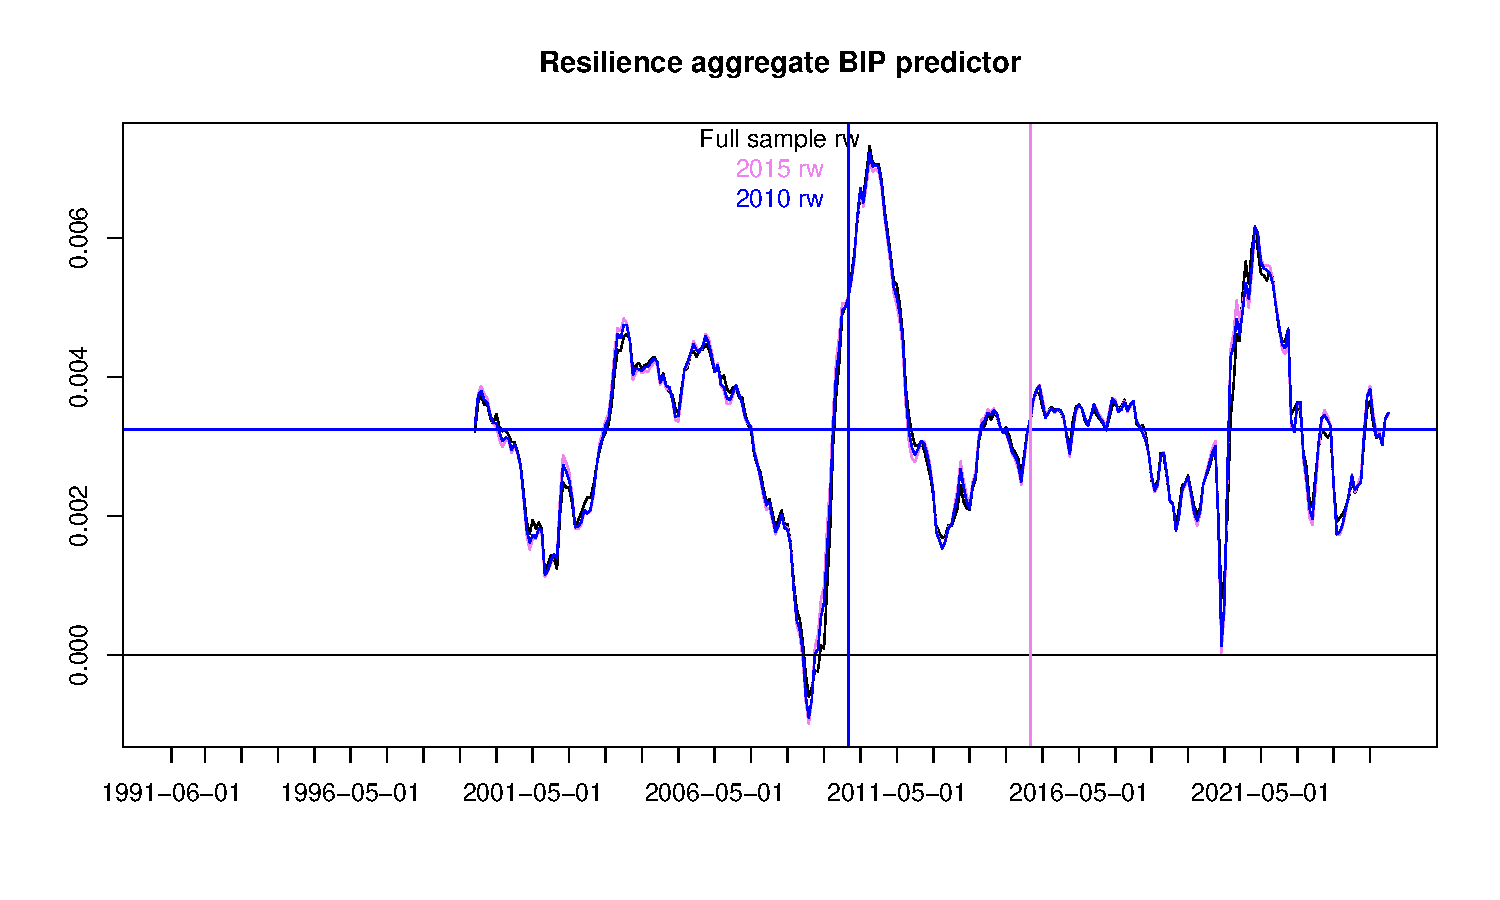
\includegraphics[height=3in, width=4in]{bip_predictor_sensitivity.pdf}\caption{Effect of look ahead delta on  left-shift/advancement of M-SSA\label{cor}}\end{center}\end{figure}\end{frame}



  






\section{Conclusion}

\frame{\sectionpage}




\begin{frame} {Conclusion}
\begin{itemize}
\item Models and performances are generally reliant on the data sample (for estimation or evaluation): `Pandemic' effect
\item Trend targets can be interpreted meaningfully in terms of economic dynamics (recessions/expansions)
\item Trend targets are easier to forecast (less noisy), see slide \eqref{slide_target_cor}
\item Multivariate designs outperform mainly with respect to trend targets and lagged series (BIP and ip), see slide \eqref{rfmse1}
\item Target correlations, sign accuracies and HT are potentially interesting alternative performance metrics
\item Target correlations and sign accuracies referenced against BIP-filter are strongly significant (not random) even on full sample (including singular Pandemic), see slides  \eqref{sample_target_cor1}, \eqref{sample_target_cor2}, \eqref{sample_target_cor3} and \eqref{sample_target_cor4}  and \eqref{signaac1}  (exception: filtered spread)
\end{itemize}
\end{frame}


\begin{frame} {Conclusion}
\begin{itemize}
\item Filters (uni and multivariate) are similar to direct AR forecasts in terms of forecast mean-square error with respect to BIP-shifted, although they do not fit the target explicitly (no overfitting), see slides \eqref{tstat1} and \eqref{slide_multi_rel_mse}
\item Real-time indicators such as {ESI} and {ifo} (any of the selected ifo series) provide additional information due to \emph{smaller publication lags} (left shifted) 
\item {Spread} is \textbf{ambiguous}:
\begin{itemize}
\item It does not appear to correlate systematically  with BIP, see CCFs on slide \eqref{ccf_pand_multe}
\item The target correlation of the corresponding M-SSA output with BIP-trend is slightly negative, see slide \eqref{sample_target_cor2}: this outcome is confirmed by the plot on slide \eqref{spr_mssa_o}
\item The t-statistics on slide \eqref{tstat1} suggest that the univariate filter based on spread tracks BIP-shifted (not BIP-trend) significantly
\item But the same univariate filter is insignificant when regressed on BIP-trend (value of the t-statistic is 1.3)
\end{itemize}
\item Models and results/outcomes are mostly interpretable (appealing)
\end{itemize}

\end{frame}


\begin{frame} {Conclusion}
\begin{itemize}
\item (M-)SSA can {control} the terms of the forecast trilemma and address user/forecast {priorities} 
\begin{itemize}
\item The {hyperparameters} ($\delta,HT)$ (HT-constraint of M-SSA) allow to {fine-tune} priorities
\item M-SSA {generalizes} classic MSE-paradigm
\end{itemize}
\item Possibility to {combine} various predictors: 
\begin{itemize}
\item {Fast} but noisier: early warning, {look ahead} indicator 
\item A bit slower but more {reliable}: nowcast, {flash} indicator 
\item Very {smooth}/reliable but retarded: {confirmatory} indicator
\end{itemize}
\item Forecast combinations: direct AR with uni- and multivariate filters
\end{itemize}

\end{frame}


\begin{frame} {Summary of (and Links to) Sample Performance Metrics}
\begin{itemize}
\item Relative \textbf{forecast mean-square} error (target: BIP-shifted): slide \eqref{rmse1} (direct AR forecasts full sample), \eqref{rmse2} (same but shorter sample), \eqref{rmse3} (univariate filters, full sample), \eqref{rmse4} (same but before Pandemic), \eqref{slide_multi_rel_mse} (multivariate filters) 

\item Relative \textbf{filter mean-square} error (target: BIP-trend): \eqref{rfmse1} (outperformance of multivariate over univariate)

\item Target \textbf{correlations}: \eqref{sample_target_cor1}, \eqref{sample_target_cor2}, \eqref{sample_target_cor3} and \eqref{sample_target_cor4} 

\item \textbf{Sign accuracies}: \eqref{signaac1} and \eqref{signaac2}

\item \textbf{t-statistics}: \eqref{tstat1},  (univariate filters and direct AR, full sample), \eqref{tstat2} (same but prior pandemic), \eqref{slide_multi_rel_mse} (multivariate filters)

\item \textbf{Holding times}: \eqref{htzc1} (direct AR and univariate filters), \eqref{htzc2} and \eqref{htzc3} (M-SSA vs. M-MSE)
\end{itemize}
\end{frame}



\begin{frame} {Design Settings (Hyperparameters) in this Study}
\begin{itemize}
\item Data: selected indicators
\item Estimation sample (for models): full data vs. ante Pandemic
\item Evaluation sample (forecast errors): full data vs. ante Pandemic
\item (V)AR(MA) model orders: ARMA(3,1), VAR(2)
\item Trend target: HP(14400)
\item (M-)SSA settings: increase of HT by $50\%$, forecast excess $\delta=0, 3, 6, 12, 18, 24$
\item Forecast horizon: $h=3$
\end{itemize}
\end{frame}


\begin{frame} {Design Settings (Hyperparameters) in this Study}
\begin{itemize}
\item Random-walk or linear interpolation of BIP: default is random walk (na.locf in read function)
\item Use two-sided HP as filter target when evaluating sample mean-square filter errors (=TRUE)
\begin{itemize}
\item One can rely on two-sided HP or on symmetrized HP-C: default is two-sided HP (T)
\end{itemize}
\item Use two-sided HP (or one-sided HP-C) as (M-)SSA/(M-)MSE targets in (M-)SSA optimization (=TRUE)
\begin{itemize}
\item One can rely on two-sided HP or on one-sided HP-C: default is two-sided HP (T)
\item One-sided HP-C is a potentially interesting target (HP-C has some interesting characteristics as a causal filter)
\end{itemize}
\end{itemize}
\end{frame}




\begin{frame} {Sources of Revisions}
\begin{itemize}
\item Data
\item Models: (V)ARMA
\item Calibration: `static' level and scale parameters
\end{itemize}
\end{frame}




\begin{frame} {To Dos}
\begin{itemize}
\item Mixed-frequency approach for BIP
\item Use all series (extension to dimension reduction and/or aggregation techniques)
\item \textbf{Better VAR(MA)}-model
\begin{itemize}
\item The weight assigned to `faster' indicators (small or no publication lag) in multi-step ahead forecasts is too weak
\end{itemize}
\item Additional forecast horizons: $h=0$ (nowcast), $h=12$ one-year forecast. 
\item Alternative holding-time constraints (smoothness)
\item Alternative filter specification(s): stronger suppression of `noisy cycles' of ifo-exp in previous plots?
\item `More' (forecast) combinations
\item Portfolio (of predictors) construction: emphasize fast/smooth tradeoff (instead of classic return/risk approach)
\item R-package, automatic up-dating with new data,...
\end{itemize}
\end{frame}



\begin{frame} {Next Steps}
\begin{itemize}
\item Worth pursuing? 
\begin{itemize}
\item Refresh (latest data)
\end{itemize}
\item Conceptual: \textbf{priorities} 
\begin{itemize}
\item Target, forecast horizon, `consensus' vs. separate predictors, ...
\end{itemize}
\item \textbf{Method}: VAR, mixed-frequency, dimension reduction,...
\item Work with \textbf{R-code} (cross-check, ROC,...): {Github}?
\item \textbf{Paper} 
\item \textbf{Application} (e.g. shiny app, public domain,...)
\end{itemize}
\end{frame}






\end{document}
